%\RequirePackage[l2tabu, orthodox]{nag}
\documentclass[11pt,a4paper]{book}
%\documentclass[11pt,a4paper]{memoir}
%\documentclass{amsbook}
%\documentclass{article}
\usepackage{amsmath, amssymb, amsthm, amsfonts}

%\usepackage{fullpage}
%\usepackage{times}
%\usepackage[squaren]{SIunits}
\usepackage[binary-units=true]{siunitx}
\usepackage{circuitikz}
\usepackage{tikz}
\usetikzlibrary{calc,patterns,decorations.pathmorphing,decorations.markings,dsp,chains}
%\usetikzlibrary{external}
%\tikzexternalize % activate!
%\tikzexternalize[prefix=tikzexternal/]
%\tikzset{external/mode=list and make}
%\tikzset{external/check=diff}
%\tikzset{external/force remake}

\usepackage{mdframed}
\usepackage{animate}

%turn animations on/off
\newif\ifanimations %default is off
\animationstrue %uncomment to turn animations on.
\ifanimations
\newcommand{\defaultframerate}{16}
\newcommand{\defaultanimation}[1]{\animategraphics[autoplay,loop]{\defaultframerate}{#1}{}{}}
\else
\newcommand{\defaultanimation}[1]{\includegraphics[page=1]{#1}}
\fi

% Define a the counter cnt. Used to identify files generated for use
% with Gnuplot.
\newcounter{cnt}
\setcounter{cnt}{0}
\makeatletter
\newcommand{\gettikzxy}[3]{%
  \tikz@scan@one@point\pgfutil@firstofone#1\relax
  \edef#2{\the\pgf@x}%
  \edef#3{\the\pgf@y}%
}
\usepackage{pgfplots}
\pgfplotsset{
compat=newest
%every axis/.append style={y tick label style={set thousands separator={}}}
}
%\usepgflibrary{fpu}
\makeatother

\usepackage[small]{caption}
\usepackage{booktabs}
\usepackage{enumitem}
\usepackage{placeins}

\bibliographystyle{robbythesis}
\usepackage[square]{natbib}

\usepackage[hidelinks]{hyperref}

% You can add more of these if it is helpful.
\theoremstyle{plain}
\newtheorem{theorem}{Theorem}
\newtheorem{definition}{Definition}
\newtheorem{lemma}{Lemma}
\newtheorem{corollary}{Corollary}
\newtheorem{result}{Result}
%\newmdtheoremenv[skipabove=\baselineskip, skipbelow=\baselineskip]{test}{Test}
\numberwithin{equation}{section}

%some math functions and symbols
\newcommand{\reals}{{\mathbb R}}
\newcommand{\ints}{{\mathbb Z}}
\newcommand{\naturals}{{\mathbb N}}
\newcommand{\complex}{{\mathbb C}}
\newcommand{\integers}{{\mathbb Z}}
\renewcommand{\Re}{\operatorname{Re}}
\renewcommand{\Im}{\operatorname{Im}}
\newcommand{\atan}[1]{\operatorname{atan}}
\newcommand{\rect}{\Pi}
\newcommand{\sinc}{\operatorname{sinc}}

\newcommand{\term}{\textbf}
\newcommand{\var}{\operatorname{var}}
\newcommand{\covar}{\operatorname{covar}}
%\newcommand{\prob}{{\mathbb P}}
\newcommand{\prob}{\operatorname{Pr}}
\newcommand{\expect}{{\mathbb E}}
\newcommand{\dealias}{\operatorname{dealias}}
\renewcommand{\mid}{\; ; \;}

% Brackets
\newcommand{\br}[1]{{\left( #1 \right)}}
\newcommand{\sqbr}[1]{{\left[ #1 \right]}}
\newcommand{\cubr}[1]{{\left\{ #1 \right\}}}
\newcommand{\scubr}[1]{{\{ #1 \}}}
\newcommand{\abr}[1]{\left< #1 \right>}
\newcommand{\abs}[1]{\left\vert #1 \right\vert}
\newcommand{\sabs}[1]{\vert #1 \vert}
 \newcommand{\floor}[1]{{\left\lfloor #1 \right\rfloor}}
\newcommand{\ceiling}[1]{{\left\lceil #1 \right\rceil}}
\newcommand{\ceil}[1]{\lceil #1 \rceil}
\newcommand{\round}[1]{{\left\lceil #1 \right\rfloor}}
\newcommand{\magn}[1]{\left\| #1 \right\|}
\newcommand{\fracpart}[1]{\left\langle #1 \right\rangle}
\newcommand{\sfracpart}[1]{\langle #1 \rangle}

\newcommand*{\calL}{\mathcal L}
\newcommand{\calD}{{\mathcal D}}
\newcommand{\calF}{{\mathcal F}}
\newcommand{\calZ}{{\mathcal Z}}

%create pgf cross shape
\usetikzlibrary{shapes.misc}

\tikzset{cross/.style={cross out, draw=black, minimum size=2*(#1-\pgflinewidth), inner sep=0pt, outer sep=0pt},
%default radius will be 1pt. 
cross/.default={1pt}
}

%tikz macros
\newcommand{\polezeroaxis}[1]{   
  \draw [<->] (-#1,0) -- (#1,0) node [above left]  {$\Re$};
  \draw [<->] (0,-#1) -- (0,#1) node [below right] {$\Im$};
 }
\newcommand{\zerotikz}[2]{ \node[draw,thick,circle,inner sep=1.75pt] at (#1,#2) {}; }
\newcommand{\poletikz}[2]{ \node[draw,thick,cross=0.1cm] at (#1,#2) {}; }

\newcommand{\vtick}[1]{\draw (#1,-0.075) -- (#1,0.075) }
\newcommand{\htick}[1]{\draw (-0.075,#1) -- (0.075,#1)}

\newcommand{\onebf}{\mathbf{1}}

%turn excersize solutions on/off
\newif\ifsolutions %default is off
%\solutionstrue %uncomment to turn solutions on.

\usepackage{comment}
\ifsolutions
  \newenvironment{solution}{\begin{footnotesize}\textbf{Solution:}}{\end{footnotesize}}
\else
  \excludecomment{solution}
\fi

\usepackage{framed,xcolor}
\definecolor{shadecolor}{gray}{0.92}
\newcommand{\todo}[1]{\textcolor{red}{TODO: #1}}
%\usepackage{shaded}

%enviroment for the practical tests (in a grey box)
\newcounter{test}
\newenvironment{test}{
\begin{shaded}\refstepcounter{test}\par\noindent%
\textbf{Test \thetest}
}{
\end{shaded}
}

%\newcommand{\mytitle}{Signals and Systems}
\ifsolutions
\newcommand{\mytitle}{Testable linear shift invariant systems (Exercise~Solutions)}
\else
\newcommand{\mytitle}{Testable linear shift invariant systems}
\fi
\title{\mytitle}
\author{Robby McKilliam}

% setup *'d (advanced) sections
% turn advanced section on/off
\newif\ifadvanced %default is off
%\advancedtrue %uncomment to turn advanced sections on.
\usepackage[pagestyles,raggedright]{titlesec}
\usepackage{titletoc}
%\usepackage{titleps}
\newcommand{\secmark}{}
\newcommand{\marktotoc}[1]{\renewcommand{\secmark}{#1}}
\ifadvanced
\newenvironment{advanced}{
  \renewcommand{\secmark}{*}%
  \addtocontents{toc}{\protect\marktotoc{*}}
}
{\addtocontents{toc}{\protect\marktotoc{}}}
\else
\excludecomment{advanced}
\fi
\titleformat{\section}{\normalfont\Large}{\makebox[1.5em][l]{\llap{\secmark}\thesection}}{0.4em}{}
\titlecontents{section}[3.7em]{}{\contentslabel[\llap{\secmark}\thecontentslabel]{2.3em}}{\hspace*{-2.3em}}{\titlerule*{}\bfseries\contentspage}
\newpagestyle{front}{%
  %\headrule
  \sethead[\thepage][][\subsectiontitle]{\sectiontitle}{}{\thepage}
  \setfoot[][][]{}{}{}
}

\newpagestyle{main}{%
  %\headrule
  \sethead[\thepage][][\mytitle]{\llap{\secmark}\thesection\quad\sectiontitle}{}{\thepage}
  \setfoot[][][]{}{}{}
}
\newpagestyle{back}{%
  %\headrule
  \sethead[\thepage][][\mytitle]{\sectiontitle}{}{\thepage}
  \setfoot[][][]{}{}{}
}

%for randomly floating stuff, e.g. the tests 
\newenvironment{randomfloat}{
\begin{figure}
}{
\end{figure}
\addtocounter{figure}{-1}
}

\newenvironment{excersizelist}{%
  \renewcommand*{\theenumi}{\thechapter.\arabic{enumi}}%
  \newcommand\itemadvanced{\stepcounter{enumi}\item[$\ast$\, \theenumi.]}
  %\renewcommand*{\theenumi}{\thechapter.\arabic{enumi}}%
  %\renewcommand*{\labelenumi}{(\arabic{enumi})}%
  \begin{enumerate}
}{%
  \end{enumerate}
}



\begin{document}

\frontmatter
\pagestyle{front}
\maketitle

\mainmatter
\pagestyle{main}

\chapter{Signals and systems}
 \section*{Exercises}

\begin{excersizelist}

\item How many distinct functions from the set $X = \{\text{Mario}, \text{Link}\}$ to the set $Y = \{\text{Freeman}, \text{Ryu}, \text{Sephiroth}\}$ exist?  Write down each function, that is, write down all functions from the set $X \to Y$.

\begin{solution}
Each of the two elements in $X$ can be mapped to one of the three elements of $Y$.  There are thus $3^2 = 9$ distinct functions in $X \to Y$.  They are
\[
f_1(x) = \begin{cases}
\text{Freeman} & x = \text{Mario} \\
\text{Freeman} & x = \text{Link} \\
\end{cases}
\qquad 
f_2(x) = \begin{cases}
\text{Freeman} & x = \text{Mario} \\
\text{Ryu} & x = \text{Link} \\
\end{cases}
\]
\[
f_3(x) = \begin{cases}
\text{Ryu} & x = \text{Mario} \\
\text{Freeman} & x = \text{Link} \\
\end{cases}
\qquad 
f_4(x) = \begin{cases}
\text{Freeman} & x = \text{Mario} \\
\text{Sephiroth} & x = \text{Link} \\
\end{cases}
\]
\[
f_5(x) = \begin{cases}
\text{Sephiroth} & x = \text{Mario} \\
\text{Freeman} & x = \text{Link} \\
\end{cases}
\qquad 
f_6(x) = \begin{cases}
\text{Ryu} & x = \text{Mario} \\
\text{Ryu} & x = \text{Link} \\
\end{cases}
\]
\[
f_7(x) = \begin{cases}
\text{Ryu} & x = \text{Mario} \\
\text{Sephiroth} & x = \text{Link} \\
\end{cases}
\qquad 
f_8(x) = \begin{cases}
\text{Sephiroth} & x = \text{Mario} \\
\text{Ryu} & x = \text{Link} \\
\end{cases}
\]
\[
f_9(x) = \begin{cases}
\text{Sephiroth} & x = \text{Mario} \\
\text{Sephiroth} & x = \text{Link} \\
\end{cases}
\]
\end{solution}

\item \label{excer:stepfunction} State whether the step function $u(t)$ is bounded, periodic, %continuous, 
absolutely integrable, an energy signal.
\begin{solution}
The magnitude of $u$ is less than or equal to one and so the signal is bounded.  The signal is not periodic, since for any hypothesised period $T > 0$ we have $u(T) = 1$ but $u(0) = 0$.  %The signal is not continuous at $t = 0$ since $\lim_{t \to 0^+} u(t) = 0$ and $\lim_{t \to 0^{-}} u(t) = 1$.  
The signal is not absolutely integrable, nor an energy signal since
\[
\|u\|_1 = \|u\|_2 = \int_{-\infty}^\infty \abs{u(t)} dt = \int_{0}^\infty dt
\]
is not finite.
\end{solution}

\item \label{exer:oneontnotlocallyint} Show that the signal $t^2$ is locally integrable, but that the signal $\frac{1}{t^2}$ is not. 

\begin{solution}
For any $a$ and $b$
\[
\int_a^b t^2 dt = \frac{b^3}{3} - \frac{a^3}{3}
\]
is finite and so $t^2$ is locally integrable.  Put $a = 0$ and $b > 0$ and
\[
\int_0^b \frac{1}{t^2} dt = -\frac{1}{b} + \lim_{t \to 0}\frac{1}{t}  = \infty.
\]
The limit above diverges and so $\frac{1}{t^2}$ is not locally integrable. 
\end{solution}

% \item \label{exer:boundedfunctionarelocallyintegrable} Show that every bounded function is locally integrable.  

\item \label{exer:functionsquarenotabsint} Plot the signal 
\[
x(t) = \begin{cases}
\tfrac{1}{t+1} & t > 0 \\
\tfrac{1}{t-1} & t \leq 0.
\end{cases}
\]
State whether it is: bounded, locally integrable, absolutely integrable, square integrable.

\begin{solution}
\begin{center}
  \begin{tikzpicture}[samples=200]
    % \draw[very thin,color=gray] (-0.1,-1.1) grid (3.9,3.9);
    \draw[->] (-4.5,0) -- (4.5,0) node[above] {$t$};
    \draw[->] (0,-1.2) -- (0,1.2);
    \draw[smooth,color=black,thick,domain=0:4] plot function{1/(x+1)};
    \draw[smooth,color=black,thick,domain=-4:0] plot function{1/(x-1)};
    \htick{1} node[pos=0.5,above right] {$1$};
    \vtick{-4} node[pos=0.5,above] {$-4$};
    \vtick{-2} node[pos=0.5,above] {$-2$};
    \vtick{2} node[pos=0.5,below] {$2$};
    \vtick{4} node[pos=0.5,below] {$4$};
  \end{tikzpicture}
\end{center}
The signal is bounded since $\abs{x(t)} < M$ for any $M > 1$.  The signal is locally integrable because it is bounded, i.e., for any finite constants $a$ and $b$
\[
\int_{a}^b \abs{x(t)} dt < \int_{a}^b M dt = (b-a)M < \infty.
\]
The signal $x$ is not absolutely integrable since
\begin{align*}
\|x\|_1 &= \int_{-\infty}^\infty \abs{x(t)} dt \\
&= 2 \int_{0}^\infty \frac{1}{t+1} dt \\
&= 2 \int_{1}^\infty \frac{1}{t} dt \\
&= 2\log(1) + \lim_{t \to \infty} 2\log(t)
\end{align*}
and the limit diverges.  The signal is square integrable since
\begin{align*}
\|x\|_2 &= \int_{-\infty}^\infty \sabs{x(t)}^2 dt \\
&= 2 \int_{0}^\infty \frac{1}{(t+1)^2} dt \\
&= 2 \int_{1}^\infty \frac{1}{t^2} dt \\
&= 2 - \lim_{t \to \infty} \frac{2}{t} = 2.
\end{align*}
\end{solution}

\item \label{excer:absintnotsquareint} Plot the signal
\[
x(t) = \begin{cases}
\frac{1}{\sqrt{t}} & 0 < t \leq 1 \\
0 & \text{otherwise}.
\end{cases}
\]
Show that $x$ is absolutely integrable, but not square integrable.

\begin{solution}
\begin{center}
  \begin{tikzpicture}[samples=50]
    % \draw[very thin,color=gray] (-0.1,-1.1) grid (3.9,3.9);
    \draw[->] (-4.5,0) -- (4.5,0) node[above] {$t$};
    \draw[->] (0,-0.2) -- (0,2.5);
    \draw[thick] (-4,0)--(0,0);
    \draw[thick,line cap=round] (1,1)--(1,0)--(4,0);
    \draw[smooth,color=black,thick,domain=0.2:1] plot function{1.0/sqrt(x)};
    \htick{1} node[pos=0.5,left] {$1$};
    \vtick{-3} node[pos=0.5,below] {$-3$};
    \vtick{-1} node[pos=0.5,below] {$-1$};
    \vtick{1} node[pos=0.5,below] {$1$};
    \vtick{3} node[pos=0.5,below] {$3$};
  \end{tikzpicture}
\end{center}
The integral
\[
\|x\|_1 = \int_{-\infty}^\infty \abs{x(t)} dt = \int_{0}^1 t^{-1/2} dt = [2\sqrt{t}]_0^1 = 2
\]
and so $x$ is absolutely integrable.  The integral
\[
\|x\|_2 = \int_{-\infty}^\infty \abs{x(t)} dt = \int_{0}^1 t^{-1} dt = [\log(t)]_0^1 = \log(1) - \lim_{t \to 0}\log(t) = \infty
\]
and so $x$ is not square integrable.
\end{solution}

\item \label{excer:energyexpchangevar} Compute the energy of the signal $e^{-\alpha^2 t^2}$ (Hint: use equation~\zeqref{eq:expabssum} on page~\zpageref{eq:expabssum} and a change of variables).
\begin{solution}
From~\zeqref{eq:expabssum} we the energy of $e^{-t^2}$ is $\sqrt{\pi}$.  Now
\[
\int_{-\infty}^\infty e^{-\alpha t^2} dt = \frac{1}{\alpha}\int_{-\infty}^\infty e^{-\tau^2} d\tau = \frac{\sqrt{\pi}}{\alpha}
\]
by the change of variables $\tau = \alpha t$.
\end{solution}

\item \label{exer:steprectnotdiff}Show that the signal $t^2$ is differentiable, but the step function $u$ and rectangular pulse $\rect$ are not.
\begin{solution}
We have
\[
\lim_{h \to 0} \frac{(t + h)^2 - t^2}{h} = \lim_{h \to 0} \frac{2 t h + h^2}{h} = 2t.
\]
\[
\lim_{h \to 0} \frac{t^2 - (t-h)^2}{h} = \lim_{h \to 0} \frac{2 t h - h^2}{h} = 2t
\]
and so $t^2$ is continuously differentiable with derivative $\frac{d}{dt} t^2 = 2t$.  At $t = 0$ the corresponding limits for the step function are
\[
\lim_{h \to 0} \frac{u(h) - u(0)}{h} = \lim_{h \to 0} \frac{0}{h} = 0
\]
but
\[
\lim_{h \to 0} \frac{u(0) - u(-h)}{h} = \lim_{h \to 0} \frac{1}{h} = \infty
\]
so the step function $u$ is not differentiable at $t = 0$.  A similar argument at $t=\tfrac{1}{2}$ or $t = -\tfrac{1}{2}$ shows that $\rect$ is not differentiable.
\end{solution}

\item \label{exer:sinplussinnotper} Plot the signal $\sin(t) + \sin(\pi t)$.  Show that this signal is not periodic.
\begin{solution}
A plot of the signal is below:

\begin{center}
\begin{tikzpicture}[domain=-1:39,xscale=0.25]
    %\draw[very thin,color=gray] (-0.1,-1.1) grid (3.9,3.9);
  \draw[->] (-2,0) -- (40,0) node[above] {$t$};
    \draw[->] (0,-2) -- (0,2) node[right] {$\sin(t) + \sin(\pi t)$};
    \draw[smooth,color=black,thick,samples=200] plot function{sin(x) + sin(pi*x)};
    %\draw[thick, dashed] (-3.4,0)--(0,0);
    %\htick{1} node[pos=0.5,left] {$0.5$};
    \vtick{10} node[pos=0.5,below] {$10$};
    \vtick{20} node[pos=0.5,below] {$20$};
    \vtick{30} node[pos=0.5,below] {$30$};
\end{tikzpicture}
%\captionof{figure}{1-dimensional continuous-time signals} \label{fig:signalsstart}
\end{center}

The following argument is due to \href{http://math.stackexchange.com/questions/1079/sum-of-two-periodic-functions}{Qiaochu Yuan}.  Suppose $\sin(t) + \sin(\pi t)$ is periodic.  Then
\[
\sin(t) + \sin(\pi t) = \sin(t + T) + \sin(\pi t + T)
\]
for some $T > 0$.  Differentiating both sides twice with respect to $t$ gives
\[
\sin(t) + \pi^2 \sin(\pi t) = \sin(t + T) + \pi^2\sin(\pi t + T)
\]
Subtracting the first equation from the second gives $\sin(t) = \sin(t + T)$ and substituting this into the second equation gives $\sin(\pi t) = \sin(\pi t + T)$.  The equation $\sin(t) = \sin(t + T)$ implies that $T = 2\pi k$ for some integer $k \neq 0$.  The equation $\sin(\pi t) = \sin(\pi t + T)$ implies that $T = 2 \ell$ for some integer $\ell \neq 0$.  We would thus have $2\pi k = 2 \ell$ and so $\pi = \tfrac{\ell}{k}$. However, this is impossible because $\pi$ is irrational.  Thus $\sin(t) + \sin(\pi t)$ is not periodic.
\end{solution}

%\item \label{exer:triangleineq} (Triangle inequality) With $a$ and $b$ complex numbers show that $\abs{a + b} \leq \abs{a} + \abs{b}$ and that $\tfrac{1}{2}\abs{a + %b}^2 \leq \abs{a}^2 + \abs{b}^2$.
%\begin{solution}
%We have
%\[
%\abs{a + b} \leq \abs{\abs{a} + \abs{b}} = \abs{a} + \abs{b}.
%\]
%Now
%\begin{align*}
%\abs{a + b}^2 &= (a+b)^*(a+b) \\
%&= \abs{a}^2 + a^* b + b^*a + \abs{b}^2 \\
%&= \abs{a}^2 + 2\Re(a^* b) + \abs{b}^2
%\end{align*}
%where $a^*$ denotes the complex conjugate and $\Re$ denotes the real part of a complex number. Now
%\[
%2\Re(a^* b) = 
%\]
%\end{solution}

\item \label{exer:L1L2linearshiftinvariant} Show that the set of locally integrable signals $L_{\text{loc}}$, the set of absolutely integrable signals $L^1$, and the set of square integrable signals $L^2$ are linear shift-invariant spaces. 
\begin{solution}
Let $x, y \in L^1$ and $a, b \in \complex$.  Now
\begin{align*}
\|a x + b y\|_1 &= \int_{-\infty}^\infty \abs{ax(t) + by(t)} dt \\
&\leq \int_{-\infty}^\infty a\abs{x(t)} + b\abs{y(t)} dt \qquad \text{triangle inequality} \\
&= a \|x\|_1 + b\|y\|_1 < \infty
\end{align*}
and so $ax + by \in L_1$ and $L_1$ is a linear space.  Also
\begin{align*}
\|T_\tau x\|_1 &= \int_{-\infty}^\infty \abs{ T_\tau x(t) } dt \\
&= \int_{-\infty}^\infty \abs{x(t - \tau)} dt \\
&= \int_{-\infty}^\infty \abs{x(k)} dk \qquad \text{change variable $k = t - \tau$}
&= \|x\|_1 < \infty
\end{align*}
and so $L_1$ is a shift-invariant space.

Now
\begin{align*}
\|a x + b y\|_2^2 &= \int_{-\infty}^\infty \abs{ax(t) + by(t)}^2 dt \\
& \int_{-\infty}^\infty \abs{a x(t)}^2 + \abs{ b y(t)}^2 + 2 \Re\big( a^* x(t)^* b y(t) \big) dt
\end{align*}
where $*$ denotes the complex cojugate and $\Re$ denotes the real part of a complex number.  Now
\[
\Re\big( a^* x(t)^* b y(t) \big) \leq \abs{a x(t)} \abs{b y(t)} \leq \max(\abs{a x(t)}^2, \abs{b y(t)}^2) \leq \abs{a x(t)}^2 + \abs{b y(t)}^2
\]
and so
\begin{align*}
\|a x + b y\|_2^2 &\leq \int_{-\infty}^\infty 3\abs{a x(t)}^2 + 3\abs{ b y(t)}^2 dt \\
&= \int_{-\infty}^\infty 3\abs{a}^2\abs{x(t)}^2 + 3\abs{b}^2\abs{ y(t)}^2 dt \\
&= 3 \abs{a}^2 \|x\|_2^2 + 3 \abs{b}^2 \|y\|_2^2 < \infty
\end{align*}
and $L_2$ is thus a linear space.  Also
\[
\|T_\tau x\|_2^2 = \int_{-\infty}^\infty \abs{ T_\tau x(t) }^2 dt = \int_{-\infty}^\infty \abs{x(t - \tau)}^2 dt = \int_{-\infty}^\infty \abs{x(t)}^2 dt = \|x\|_2^2 < \infty
\]
and so $L_2$ is a shift-invariant space.
\end{solution}

\item \label{exer:periodicshiftinvariantnotlinear} Show that the set of periodic signals is a shift-invariant space, but not a linear space.
\begin{solution}
Let $P$ be the set of periodic signals.  If $x \in P$ then there exists $T > 0$ such that $x(t + kT) = x(t)$ for all $t \in \reals$ and $k \in \ints$.  The shifted signal $T_\tau x \in P$ since, for the same $T$, we have
\[
T_\tau x(t - kT) = x(t - \tau - kT) = x(t - \tau) = T_\tau x(t)
\]
for all $t \in \reals$ and all $k \in \ints$.  Since $x \in P$ and $\tau \in \reals$ are arbitrary, this holds for all signals $x \in P$ and all shifts $\tau \in reals$.   Thus, the set of periodic signals is a shift invariant space.

The set of period signals is not a linear space.  Consider the signal $x(t) = \sin(t)$ with period $2\pi$ and $y(t) = \sin(\pi t)$ with period $2$.  Both $x$ and $y$ are in $P$.  However, exercise~\ref{exer:sinplussinnotper} shows that the sum $x(t) + y(t) = \sin(t) + \sin(\pi t)$ is not periodic, that is, $x + y \in P$.
\end{solution}

\item \label{exer:boundedlinearshiftinvar} Show that the set of bounded signals is a linear shift-invariant space.
\begin{solution}
Let $B$ be the set of bounded signals.  If $x \in B$ there exists $M > 0$ such that $\abs{x(t)} < M$ for all $t \in \reals$ then the shift $T_\tau x(t)$ satisfies $\abs{T_\tau x(t)} < M$ for all $t \in \reals$.  Since $x$ and $\tau$ are arbitrary this holds for all $x \in B$ and $\tau \in \reals$.  Thus $B$ is a shift invariant space.

Let $x \in B$ and $y \in B$ be bounded signals.  There exists $M_x > 0$ and $M_y > 0$ such that
\[
\abs{x(t)} < M_x \qquad \abs{y(t)} < M_y \qquad \text{for all $t \in \reals$}.
\]
Now for $a, b \in \complex$ the signal $ax + by$ satisfies
\[
\abs{ax(t) + by(t)} \leq \abs{a}\abs{x(t)} + \abs{b}\abs{y(t)} < \abs{a} M_x + \abs{b} M_y
\]
for all $t \in \reals$.  Thus the linear combination $ax+by$ is bounded.  Since $a,b \in \complex$ and $x,y \in B$ are arbtirary this holds for all $a,b \in \complex$ and all $x,y \in B$ and so $B$ is a linear space. 
\end{solution}

\item \label{exer:boundconstantnotlinear} Let $K > 0$ be a fixed real number. Show that the set of signals bounded below $K$ is a shift invariant space, but not a linear space. 
\begin{solution}

\end{solution} 

\item \label{exer:evenoddnoshiftinvariant} Show that the set of even signals and the set of odd signals are not shift invariant spaces.

\item \label{excer:integratornotstable1} Show that the integrator $I_c$ with finite $c\in\reals$ is not stable.
\begin{solution}
Put $M > 1$.  The shifted step function $u(t + a)$ is locally integrable and bounded below $M$, i.e. $\sabs{u(t+a)} \leq 1 < M$ for all $t \in \reals$.  However, the response of the integrator $I_a$ to $u(t+a)$ is
\[
I_au(t+a) = \int_{-a}^t u(\tau + a)d\tau = \begin{cases}
\int_{-a}^t d\tau = t + a & t \geq -a \\
0 & t < -a 
\end{cases},
\]
and this is not a bounded signal, that is, for every $K$ we have $t + a > K$ whenever $t > K - a$.
\end{solution}

\item \label{excer:domainintegrator} Show that if the signal $x$ is locally integrable and $\int_{-\infty}^0\abs{x(t)}dt < \infty$ then $I_\infty x(t) = \int_{-\infty}^t x(t) dt < \infty$ for all $t \in \reals$.
\begin{solution}
We have
\begin{align*}
I_\infty x(t) \leq \abs{I_\infty x(t)} &= \abs{\int_{-\infty}^t x(t)dt } \\
&\leq \int_{-\infty}^t \abs{x(t)}dt \\
&= \int_{-\infty}^0 \abs{x(t)}dt + \int_{0}^t \abs{x(t)}dt
\end{align*}
Now $\int_{-\infty}^0 \abs{x(t)}dt < \infty$ by assumption and $\int_{0}^t \abs{x(t)}dt$ because $x$ is locally integrable.  It follows that 
\end{solution}

\item \label{excer:integratornotstable} Show that the integrator $I_\infty$ is not stable.
\begin{solution}
By default the domain for $I_\infty$ is the subset of locally integrable signals for which $\int_{-\infty}^0\abs{x(t)}dt < \infty$.  The step function $u(t)$ is in this domain.  The argument now follows similiarly to Exercise~\ref{excer:integratornotstable}.
\end{solution}

\item \label{excer:diffnotstable} Show that the differentiator system $D$ is not  stable.
\begin{solution}
Put $M > 2$.  Define the signal
\[
q_a(t) = \begin{cases}
0 & 2t < -a \\
1 + \sin\big(\tfrac{\pi t}{a}\big) & -a < 2t < a \\
2 & 2t > a,
\end{cases}
\]
and observe that $q_a$ is differentiable and bounded below $M$.  The response of the differentiator $D$ to $q_a$ is
\[
Dq_a(t) = \begin{cases}
0 & 2t < -a \\
\tfrac{\pi}{a} \cos\big(\tfrac{\pi t}{a}\big) & -a < 2t < a \\
1 & 2t > a.
\end{cases}
\]
The signal $p_a$ and the response $Dp_a$ are plotted below for $a = \tfrac{1}{2},1$ and $2$.  The response $Dp_a$ obtains a maximum amplitude of $\tfrac{\pi}{a}$ at $t=0$.  So $D$ is not stable because for any $K$ we can choose $a < \tfrac{\pi}{K}$ so that $\tfrac{\pi}{a} > K$.

\newcommand{\sinpulse}[1]{
\draw[color=black,thick] (-1.5,0) -- (-#1/2,0) node {};
\draw[smooth,color=black,thick,domain=-#1/2.0:#1/2.0] plot function{1 + sin(3.14159265359*x/#1)};
\draw[color=black,thick] (#1/2,2) -- (1.5,2)  node {};
}
\newcommand{\responsesinpulse}[1]{
\draw[color=black,thick] (-1.5,0) -- (-#1/2,0) node {};
\draw[smooth,color=black,thick,domain=-#1/2.0:#1/2.0] plot function{3.14159265359/#1*cos(3.14159265359*x/#1)};
\draw[color=black,thick] (#1/2,0) -- (1.5,0)  node {};
}
\newcommand{\sinpulseresponse}[1]{}
\begin{center}
  \begin{tikzpicture}
    % \draw[very thin,color=gray] (-0.1,-1.1) grid (3.9,3.9);
    \draw[->] (-2,0) -- (2,0) node[above] {$t$};
    \draw[->] (0,-0.5) -- (0,2.5) node[right] {$q_a(t)$};
    \sinpulse{1};
    \sinpulse{0.5};
    \sinpulse{2};
  \end{tikzpicture}
\;\;
  \begin{tikzpicture}
    \begin{scope}[yscale=0.5]
    % \draw[very thin,color=gray] (-0.1,-1.1) grid (3.9,3.9);
    \draw[->] (-2,0) -- (2,0) node[above] {$t$};
    \draw[->] (0,-1) -- (0,7) node[right] {$Dq_a(t)$};
    \responsesinpulse{1};
    \responsesinpulse{0.5};
    \responsesinpulse{2};
    \end{scope}
  \end{tikzpicture}
\end{center}


Another solution was suggested by Badri Vellambi.  Consider the signal $x(t) = \sin( t^2)$ plotted in the figure below.  This signal is bounded below any $M > 1$.  The response of the differentiator is $Dx(t) = 2t \cos(t^2)$ and this is not bounded.

\begin{center}
  \begin{tikzpicture}
    \begin{scope}[yscale=2,xscale=0.4]
    % \draw[very thin,color=gray] (-0.1,-1.1) grid (3.9,3.9);
    \draw[->] (-6,0) -- (6,0) node[above] {$t$};
    \draw[->] (0,-1.5) -- (0,1.5) node[right] {$\sin(t^2)$};
    \draw[smooth,color=black,thick,domain=-5.5:5.5,samples=200] plot function{sin(x*x)};
    \end{scope}
  \end{tikzpicture}
\;\;
  \begin{tikzpicture}
    \begin{scope}[xscale=0.4]
    % \draw[very thin,color=gray] (-0.1,-1.1) grid (3.9,3.9);
    \draw[->] (-6,0) -- (6,0) node[above] {$t$};
    \draw[->] (0,-3) -- (0,3) node[right] {$2t \cos(t^2)$};
    \begin{scope}[yscale=0.25] 
      \draw[smooth,color=black,thick,domain=-5.5:5.5,samples=200] plot function{2*x*cos(x*x)};
    \end{scope}
    \end{scope}
  \end{tikzpicture}
\end{center}

\end{solution}


\item Show that the shifter $T_\tau$ is linear and shift-invariant and that the time-scaler is linear, but not time invariant.
\begin{solution}
The shifter $T_\tau$ is shift-invariant since
\[
T_kT_\tau x  = T_kx(t - \tau) = x(t - \tau - k) = T_\tau x(t - k) = T_\tau T_k x 
\]
for all signals $x$, that is, shifters commute with shifters.  The shifter is linear because
\[
T_\tau(ax + by) = ax(t - \tau) + by(t - \tau) = a T_\tau x + b T_\tau y.
\]
The time-scaler $H x = x(\alpha t)$ is linear because
\[
H(ax + by) = ax(\alpha t) + by(\alpha t) = aHx + b Hy.
\]
The system is not shift-invariant because
\[
HT_\tau x = Hx(t-\tau) = x(\alpha t - \tau)
\]
but 
\[
T_\tau H x = T_\tau x(\alpha t) = x(\alpha(t - \tau)) = x( \alpha t - \alpha \tau ),
\]
and these signals are not equal in general.  For example consider the rectangular pulse $\Pi$.  With time-scaling parameter $\alpha = 2$ and shift $\tau = 1$,
\[
H T_1 \Pi = \Pi( 2 t - 1 ) \neq \Pi( 2t - 2 ) = T_1 H \Pi .
\]
\end{solution}

%\item \label{excer:difflLTI} Show that the $k$th differentiator $D^k(x,t) = \tfrac{d^k}{dt^k} x(t)$ is linear and time-invariant

\item Show that the integrator $I_c$ with finite $c \in \reals$ is linear, but not shift-invariant.
\begin{solution}
The system is linear because, if $x, y \in L_{\text{loc}}$, then
\begin{align*}
I_c(ax + by) &= \int_{-c}^t ax(\tau) + b y(\tau) d\tau \\
&= a\int_{-c}^t x(\tau) d\tau + b \int_{-c}^t y(\tau) d\tau \\
&= a I_c x  + b I_c y.
\end{align*}
The system is not shift-invariant because
\[
T_k I_c x = I_c(x,t-k) = \int_{-c}^{t-k} x(\tau) d\tau 
\]
but
\[
I_c T_k x = \int_{-c}^{t} x(\tau-k) d\tau.
\]
We now need only find some signal $x \in L_{\text{loc}}$ for which the integrals on the right hand side of the above equations are not equal.  Choose the signal $x = 1$, i.e., the signal that is equal to $1$ for all time.  In this case
\[
T_k I_c 1 = \int_{-c}^{t-k} d\tau =  t-k+c \neq t + c = \int_{-c-k}^{t-k} d\tau = I_c T_k 1 \qquad \text{when $k \neq 0$.}
\]
\end{solution}

\item Show that the integrator $I_\infty$ is linear and shift-invariant.
\begin{solution}
The system is linear because
\begin{align*}
I_\infty(ax + by) &= \int_{-\infty}^t ax(\tau) + b y(\tau) d\tau \\
&= a\int_{-\infty}^t x(\tau) d\tau + b \int_{-\infty}^t y(\tau) d\tau \\
&= a I_\infty x   + b I_\infty y .
\end{align*}
The system is shift-invariant because
\[
T_k I_\infty x = I_\infty x(t-k) = \int_{-\infty}^{t-k} x(\tau) d\tau,
\]
and
\[
I_\infty T_k x = \int_{-\infty}^{t} x(\tau-k) d\tau = \int_{-\infty}^{t-k} x(\tau) d\tau.
\]
\end{solution}

\item State whether the system $H x = x + 1$ is linear, shift-invariant, stable.
\begin{solution}
It is not linear because for any signal $x$ and real number $a \neq 1$,
\[
H(ax) = ax + 1 \neq aH x = a\big( x + 1\big) = ax + a.
\]
It is shift-invariant because
\[
H T_{\tau} x  = x(t - \tau) + 1 = T_\tau(x + 1) = T_\tau H x.
\]
It is  stable because for any signal $x$ with $x(t) < M$ for all $t\in\reals$, 
\[
Hx(t) = x(t) + 1 < M+1 \qquad \text{for all $t \in \reals$}. 
\]
\end{solution}

\item State whether the system $H x = 0$ is linear, shift-invariant,  stable.
\begin{solution}
It is linear because
\[
H(ax + by) = 0 = aH x + bH y = 0.
\]
It is shift-invariant because
\[
H T_{\tau} x (t) = 0 = H x(t-\tau).
\]
It is stable because for any $K > 0$,
\[
Hx(t) = 0 < K \qquad \text{for all $t \in \reals$ and all signals $x$}. 
\]
\end{solution}

\item State whether the system $Hx = 1$ is linear, shift-invariant,  stable.
\begin{solution}
It is not linear because for any signal $x$ and real number $a \neq 1$
\[
H(ax) = 1 \neq  aHx = a.
\]
It is shift-invariant because
\[
HT_{\tau} x = 1 = T_\tau(1) = T_\tau Hx.
\]
It is  stable because for any $K > 1$, 
\[
\abs{H x(t)} = 1 < K \qquad \text{for all $t \in \reals$ and all signals $x$}. 
\]
\end{solution}

\item \label{exer:periodnotabsint} Let $x$ be a signal with period $T$ that is not equal to zero almost everywhere.  Show that $x$ is neither absolutely integrable nor square integrabl.
\begin{solution}
This is plain and does not really require further explanation, but I've found some students desire more rigour.  

Since $x$ does not equal to zero almost everywhere there exist some finite real numbers $a$ and $b$  such that $\int_{a}^b \abs{x(t)}dt = C > 0$.  Let $k$ be an integer such $-kT < a$ and $kT > b$ so that the integral over $2k+1$ periods 
\[
\int_{-kT}^{kT}\abs{x(t)}dt \geq \int_{a}^b \abs{x(t)}dt = C > 0.
\] 
Now, since $x$ has period $T$
\[
\int_{-ckT}^{ckT}\abs{x(t)}dt = (2c+1) \int_{-kT}^{kT}\abs{x(t)}dt \geq (2c+1)C > 0
\] 
for integers $c$ and since this integral is increasing monotonically with $c$ we have $\int_{-ckT}^{ckT}\abs{x(t)}dt \geq \floor{2c+1}C$ for all $c \in \reals$ where $\floor{2c+1}$ denotes the largest integer less than or equal to $2c+1$.  Now,
\[
\|x\|_1 = \int_{-\infty}^{\infty} \abs{x(t)} dt = \lim_{c \to \infty} \int_{-ckT}^{ckT}\abs{x(t)}dt \geq \lim_{c \to \infty} \floor{2c+1}C = \infty,
\]
and so, $x$ is not absolutely integrable.

%BLERG.  A similar approach can be used to show that x is not square integrable, but you need to use that the function spaces $L^2(T) \subset L^1(T)$ to get an equivalent constant $C$ from assumptions of $x\neq 0 a.e.$.
\end{solution}

\end{excersizelist}

% Start your notes here.
%BLERG: TO DO
% Potentially add to Section 1, definition of limit, continuity, absolute continuity, convergence of signal (pointwise and uniform), and continuity of systems (pointwise, uniform etc).
% We assume/hypothesise that practical systems (electrical, mechanical etc)  are linear and shift invariant.  This does not follow from the differential equations.  It's a hypothesis that should be tested like any other.  It's also likely necessary to assume continuity and single valuedness,   See Zemanian Chapter 10 - Passive Systems.  It might be worth writting something on this.


%%% Local Variables: 
%%% mode: latex
%%% TeX-master: "main.tex"
%%% End: 


\chapter{Systems modelled by differential equations}\label{sec:syst-modell-diff}
 
\section*{Exercises}

\begin{excersizelist}

\item \label{exer:multiplieropampwithmodel}  Analyse the inverting amplifier circuit in Figure~\zref{circ:opampinvertingamplifierequivalent} to obtain the relationship between input voltage $x$ and output voltage $y$ given by~\zeqref{eq:intertingopampmodel}.  You may wish to use a symbolic programming language (for example Maxima, Sage, Mathematica, or Maple).
\begin{solution}
We provide two solutions.  Let $v_i$, $v_o$, $v_1$ and $v_2$ be the voltages over the input resistor $R_i$, the output resistor $R_o$, and resistors $R_1$ and $R_2$ respectively.  Observe that $v_+ - v_i = v_i$ and so the voltage over the dependent source is $A v_i$.  The voltages satisfy,
\begin{align*}
x &= v_1 - v_i \\
y &= -v_i - v_2 \\
y &=  v_o + Av_i
\end{align*}
The currents into the 3 way connection between $R_i, R_1$ and $R_2$ sum to zero, and so
\[
\frac{v_1}{R_1} + \frac{v_i}{R_i} = \frac{v_2}{R_2}
\]
by Ohm's law, the direction of current moving from positive to negative voltage.  Finally the currents through $R_o$ and $R_2$ are the same, and so
\[
\frac{v_o}{R_o} = \frac{v_2}{R_2}.
\]
We now have 5 linearly independent equations for the six unknowns $v_1, v_2, v_o, v_i, x, y$.  We can use these to find an equation that describes $y$ in terms of $x$.  The Mathematica command
\begin{verbatim}
Simplify[Solve[{x == v1 - vi,
   y == vo + A*vi,
   y == -vi - v2,
   v1/r1 + vi/ri == v2/r2,
   vo/ro == v2/r2,
   r1 > 0, r2 > 0, ro > 0, ri > 0, A > 0},
  {y, vi, vo, v2, v1}, Reals]]
\end{verbatim}
or Maxima command
\begin{verbatim}
linsolve([x = v1 - vi,
   y = vo + A*vi,
   y = -vi - v2,
   v1/r1 + vi/ri = v2/r2,
   vo/ro = v2/r2],
   [y, vi, vo, v2, v1]);
\end{verbatim}
readily obtains
\[
y = \frac{R_i (R_o - A R_2) }{R_i (R_2+R_o)+R_1 (R_2+R_i + A R_i+R_o)}x.
\]

The second solution is thanks to Badri Vellambi.  Consider the operational amplifier circuit with feedback presented in Fig.~\ref{Fig-Prob2.1a}. Suppose that the voltage signal fed into the circuit is $x(t)$ and the voltage signal measured at the output of the opamp is $y(t)$. 

{
\centering
\captionsetup{type=figure}
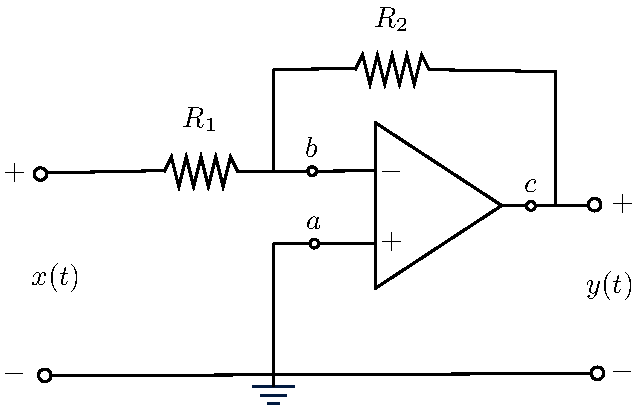
\includegraphics[width=3in]{plots/multiplierbadri1.pdf}
\captionof{figure}{The circuit}
 \label{Fig-Prob2.1a}
}

To simplify the circuit, one has to use the model for the opamp given in Fig.~\ref{Fig-Prob2.1b} which involves the voltage-controlled voltage-source (VCVS) at the output side (indicated in green).  While replacing the operational amplifier with its model, it must be noted that the positive terminal of the operational amplifier is connected to the ground.

{
\centering 
\captionsetup{type=figure}
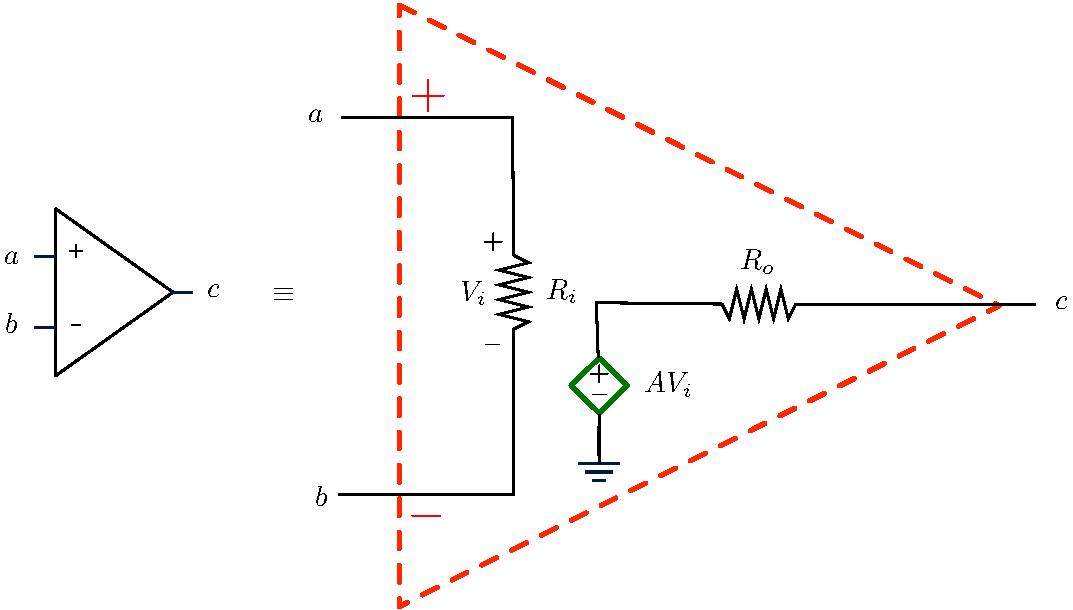
\includegraphics[width=5in]{plots/multiplierbadri2.pdf}
\captionof{figure}{The model for an operational amplifier}
 \label{Fig-Prob2.1b}
}

Upon replacement, we obtain the following equivalent circuit. Again notice that since the positive terminal of the opamp was connected to the ground, the voltage output by the VCVS is $AV_i$ where $V_i$ is the voltage between the ground and the top of the resistance $R_i$, and is measured against the flow of the current $i-i_1$ as is indicated in the figure.

{
\centering 
\captionsetup{type=figure}
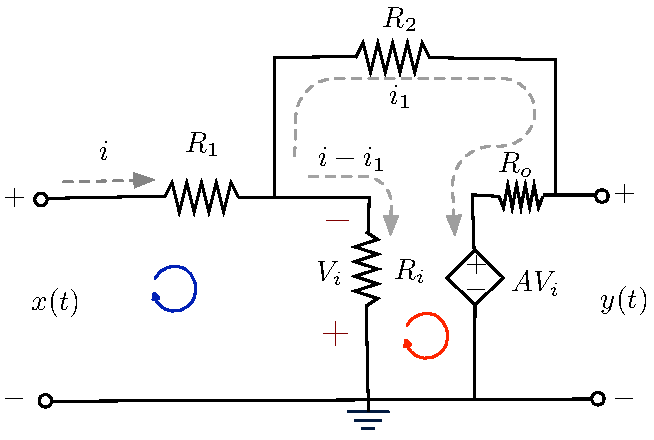
\includegraphics[width=4in]{plots/multiplierbadri3.pdf}
\captionof{figure}{The operational amplifier circuit with the model}
 \label{Fig-Prob2.1c}
}

Applying Kirchoff's law to the outer loop indicated in blue in Fig.~\ref{Fig-Prob2.1c}, we obtain the following equation.
\begin{equation}
x(t) = iR_1+(i-i_1)R_i = i(R_1+R_i) - i_1 R \label{eqn-Prob2.1.1}
\end{equation}
Note that by definition, the voltage $V_i$ that controls the VCVS is the voltage across $R_i$ measured against the indicated direction of the current $i-i_1$, and is given by
\begin{equation}
V_i = -(i-i_1)R_i. \label{eqn-Prob2.1.2}
\end{equation}
Next, writing out the Kirchoff's law for the inner loop indicated in red, we obtain the following.
\begin{align}
0 &= i_1 R_2 + i_2 R_0 + AV_i - (i-i_1) R_i
\end{align}
Substituting $V_i$ in the above equation with the RHS of \eqref{eqn-Prob2.1.2}, we obtain the following.
\begin{align}
0&= i_1 (R_2+R_0) - A(i-i_1)R_i-(i-i_1)R_i\\
&= -i(1+A)R_i+i_1((1+A)R_i+R_0+R_2)\label{eqn-Prob2.1.3}
\end{align}
Combining \eqref{eqn-Prob2.1.3} and \eqref{eqn-Prob2.1.1}, we obtain the following linear system of equations governing the electrical circuit.
\begin{align}
\left[\begin{array}{cc} R_1+R_i &  -R_i\\ -(1+A)R_i & (1+A)R_i+R_0+R_2\end{array}\right]\left[\begin{array}{c} i\\ i_1\end{array}\right] = \left[\begin{array}{c} x(t)\\ 0\end{array}\right]
\end{align}
Solving the above linear system, we identify the current in the different branches to be
\begin{align}
\left[\begin{array}{c} i\\ i_1\end{array}\right] = x(t)\left[\begin{array}{c} \frac{ (1+A)R_i+R_0+R_2}{(1+A) R_iR_1+R_0R_1+R_2R_1+R_0R_i+R_2R_i}\\ \frac{(1+A)R_i}{(1+A) R_iR_1+R_0R_1+R_2R_1+R_0R_i+R_2R_i}\end{array}\right].\label{eqn-Prob2.1.4}
\end{align}
Lastly, notice that
\begin{align}
y(t) &= i_1 R_0 + A V_i \\
 & = i_1 R_0 - (i-i_1)R_i.
\end{align}
Substituting the solutions for $i$ and $i_1$ in terms of $x(t)$, we obtain the following.
\begin{align}
y(t)= \left( \frac{R_iR_0 - R_2R_iA}{(1+A) R_iR_1+R_0R_1+R_2R_1+R_0R_i+R_2R_i} \right)x(t)
\end{align}


\end{solution}


\item \label{exer:twomassspringtwowalls} Figure~\ref{mech:twomassspringtwowalls} depicts a mechanical system involving two masses, two springs, and a damper connected between two walls.  Suppose that the spring $K_2$ is at rest when the mass $M_2$ is at position $p(t) = 0$.  A force, represented by the signal $f$, is applied to mass $M_1$.  Derive a differential equation relating the force $f$ and the position $p$ of mass $M_2$.

\begin{solution}
Let $p_1$ be a signal representing the position of mass $M_1$.  Suppose that the spring $K_1$ connecting masses $M_1$ and $M_2$ is a rest when the masses are distance $d_1$ apart, i.e., $p - p_1 = d_1$.  The force applied by the spring on $M_2$ is by spring $K_1$ is 
\[
f_1 = -K_1(p - p_1 - d_1) = -K_1(p - g)
\] 
where $g = p_1 + d_1$.  The force applied by spring $K_1$ on mass $M_1$ is then $-f_1$.  The force applied by the damper on $M_1$ is
\[
f_d = -BD p_1 = -BD(g - d_1) = - BD g.
\]
The total force applied to $M_1$ is $f + f_d - f_1$ and by Newton's law
\[
M_1 D^2 p_1 = M_1 D^2g = f + f_d - f_1 = f - BDg + K_1(p - g).
\]
The force applied to $M_2$ by the spring $K_2$ is
\[
f_2 = -K_2 p 
\] 
because the spring is assumed to be at rest when $p = 0$.  The total force applied to $M_2$ is $f_1 + f_2$ and by Newton's law
\[
M_2 D^2p = f_1 + f_2 =  -K_1(p - g) - K_2p.
\]
Rearranging gives
\[
-K_1 g = (K_1+K_2)p + M_2 D^2p
\]
and
\[
-K_1(p - g) = M_2 D^2p  + K_2p .
\]
Now,
\[
M_1 D^2g + BDg + M_2 D^2p  + K_2p = f 
\]
and so
\[
K_1K_2 p + B(K_1+K_2)Dp + (M_1K_1 + M_1K_2 + K_1 M_2) D^2p  + BM_2D^3p + M_1M_2 D^4p = K_1 f .
\]
In the case that $M_1 = K_1 = K_2 = B = 1$ and $M_2 = 2$ we have
\[
p + 2Dp + 4D^2p + 2D^3p + 2D^4p = f.
\]
\end{solution}

\begin{figure}[p]
\centering
\begin{tikzpicture}
\tikzstyle{spring}=[thick,decorate,decoration={coil,pre length=0.3cm,post length=0.3cm,segment length=6,aspect=0.9}]
\tikzstyle{damper}=[thick,decoration={markings,  
  mark connection node=dmp,
  mark=at position 0.5 with 
  {
    \node (dmp) [thick,inner sep=0pt,transform shape,rotate=-90,minimum width=15pt,minimum height=3pt,draw=none] {};
    \draw [thick] ($(dmp.north east)+(2pt,0)$) -- (dmp.south east) -- (dmp.south west) -- ($(dmp.north west)+(2pt,0)$);
    \draw [thick] ($(dmp.north)+(0,-5pt)$) -- ($(dmp.north)+(0,5pt)$);
  }
}, decorate]
\tikzstyle{ground}=[fill,pattern=north east lines,draw=none,minimum width=0.75cm,minimum height=0.3cm]
\tikzstyle{wall}=[fill,pattern=north east lines,draw=none,minimum width=0.3cm,minimum height=2cm]

\node (Wleft) [wall] {};
\draw (Wleft.north east)--(Wleft.south east);

\node (M1) [minimum width=1cm,minimum height=2cm,style={draw,outer sep=0pt,thick},xshift=2.65cm] {$M_1$};
\draw [damper] (Wleft.east)--(M1.west) node[pos=0.5,above,minimum height=30pt] {$B$};
%\draw [-latex,thick] (M1.north) ++(-0.5cm,0.3cm) -- +(1cm,0) node[pos=0.5,above] {$f(t)$};
\draw [-latex,thick] (M1.south) ++(-0.5cm,-0.3cm) -- +(1cm,0) node[pos=0.5,below] {$f(t)$};

\node (M2) [minimum width=1cm,minimum height=2cm,style={draw,outer sep=0pt,thick},xshift=5.15cm] {$M_2$};
\draw [spring] (M1.east)--(M2.west) node[pos=0.5,above,minimum height=20pt] {$K_1$};
\draw [-latex,thick] (M2.south) ++(-0.5cm,-0.3cm) -- +(1cm,0) node[pos=0.5,below] {$p(t)$};

\node (Wright) [wall,xshift=7.8cm] {};
\draw (Wright.north west)--(Wright.south west);
\draw [spring] (M2.east)--(Wright.west) node[pos=0.5,above,minimum height=20pt] {$K_2$};
%\draw [thick,<->] (Wleft.north east)++(0,0.25cm) -- ++(7.5cm,0) node[pos=0.5,above] {$d$};

\end{tikzpicture}
\caption{Two masses, a spring, and a damper connect between two walls for Exercise~\ref{exer:twomassspringtwowalls}.} \label{mech:twomassspringtwowalls}
\end{figure}



\item \label{exer:dcmotorpotfeedback} Consider the electromechanical system in Figure~\ref{fig:dcmotorpotfeedback}.  A direct current motor is connected to a potentiometer in such a way that the voltage at the output of the potentiometer is equal to the angle of the motor $\theta$.  This voltage is fed back to the input terminal of the motor.  An input voltage $v$ is applied to the other terminal on the motor.  Find the differential equation relating $v$ and $\theta$.  What is the input voltage $v$ if the motor angle satisfies $\theta(t) = \frac{\pi}{2} (1 + \operatorname{erf}(t) )$?  Plot $\theta$ and $v$ in this case when the motor coefficients satisfy $L=0$, $R = \tfrac{3}{4}$, and $K_b=K_\tau=B=J=1$.
%Find the transfer function of the system that maps the input voltage $v$ to the motor angle $\theta$.  %Under the assumption that the motor coefficients satisfy $L=0$ and $K_b=K_\tau=B=R=J=1$ draw a pole zero plot and determine whether this system is stable and/or regular.  Find and plot the impulse response and step response if they exist.

{
\begin{figure}[tp]
  \centering
  \newcommand{\arcdegree}{25}
  \begin{circuitikz} \draw
    (4,0) to[open] (4,3) to[R, l=$R$,-o] (0,3);
    %to[short] (0,4);
    %to[short] (7.75,4) to[short,-o] (7.75,1.5);
    \draw (7,2.5) to[potentiometer,*-*] (7,0.5);
    \draw (0,-1) to[open, v^>=$v$,o-o] (0,3);
    \draw (7.75,1.5) to[short] (7.75,0) to[short] (4,0);
    \draw (7.5,1.5) to[short,-o] (9,1.5);
    %\draw (3,-1) node[ground] {};
    \draw (0,-1) to[short] (9,-1) to[open,o-o,v>=$\theta$] (9,1.5);
    \begin{scope}[xshift=4cm,yshift=1.5cm]
      \node (M) [circle,style={draw,thick}] {motor};
      \node [right of=M, minimum width=1cm,rectangle,style={draw,thick},node distance=1.8cm] (J) {$J$};
      \draw (M.east) -- (J.west);
      \draw [->,>=stealth'] (J.east) -- +(0.4cm,0) node[] {};
      \draw [-latex] (M.west) ++(-0.2cm,-0.5cm) -- +(0cm,1.0cm) node[pos=0.5,left] {$v_b$};
      \draw (M.north) -- (0,3-1.5);
      \draw (M.south) -- (0,0-1.5);
      \begin{scope}[yshift=1cm,xshift=0.8cm]
        \draw [latex-,thick] (\arcdegree:1) arc (\arcdegree:-\arcdegree:1);
        \node at (0:1) [right] {$\theta$};
      \end{scope}
    \end{scope}
  \end{circuitikz}
  \caption{Diagram for a rotary direct current (DC) with potentiometer feedback for Exercise~\ref{exer:dcmotorpotfeedback}.} \label{fig:dcmotorpotfeedback}
\end{figure}
}

\begin{solution}
The input voltage to the DC motor is $v - \theta$.  From~(\zref{eq:dcmotordiffequation}) of the lecture notes the relationship between the input voltage and motor angle is
\[
v - \theta = \left(\frac{RB}{K_\tau} + K_b\right) D\theta + \frac{RJ}{K_\tau} D^2\theta
\] 
and so
\[
v = \theta + \left(\frac{RB}{K_\tau} + K_b\right) D\theta + \frac{RJ}{K_\tau} D^2\theta.
\]
If $\theta(t) = \frac{\pi}{2} (1 + \operatorname{erf}(t) )$ then
\[
D\theta(t) = \sqrt{\pi} e^{-t^2}, \qquad D^2\theta(t) = -2t \sqrt{\pi} e^{-t^2}
\]
and so
\[
v(t) = {{\pi\,\left(\mathrm{erf}\left(t\right)+1\right)}\over{2}}-2\,
 \sqrt{\pi}\,t\,e^ {- t^2 }+2\,\sqrt{\pi}\,e^ {- t^2 }
\]
The signals $v$ and $\theta$ are plotted in the figure below.  Observe that as $t \to \infty$ both $\theta(t)$ and $v(t)$ converge to $\pi$.

\begin{figure}[tp]
  \centering
  \defaultanimation{tikzfigs/dcmotorstabilised}
%\animategraphics[autoplay,loop,every=\every]{\defaultframerate}{}{}{}
  \caption{Voltage and corresponding angle for the dc motor with potentiometer in Figure~\ref{fig:dcmotorpotfeedback} with constants $L =0$, $R = \tfrac{3}{4}$, and$K_b=K_\tau=B=J=1$.} \label{fig:dcmotorpotfeedbackdcmotoranim}
\end{figure}


% The transfer function is
% \[
% \frac{\calL(v)}{\calL(\theta)} = \frac{1}{1 + \left(\frac{RB}{K_\tau} + K_b\right) s  + \frac{RJ}{K_\tau} s^2}.
% \]
% Under the assumption that $K_b=K_\tau=B=R=J=1$ the transfer function is
% \[
% \frac{\calL(v)}{\calL(\theta)} = \frac{1}{1 + 2s  + s^2} = \frac{1}{(1 + s)^2}.
% \]
% There are two equal real poles at $s = -1$ and no zeros.  A pole zero plot is below.

% \begin{center}
%   \begin{tikzpicture}
%     \poletikz{-1}{0} \node[below] at (-1,0) {$-1$};
%     \polezeroaxis{2}
%   \end{tikzpicture}
% \end{center}

% The system is regular because there are more poles than zeros.  The system is stable because there are at least as many poles as zeros and all poles have negative real part.  The impulse response is found to be $h(t) u(t) t e^{-t}$ by application of the inverse Laplace transform.  The step response is given by application of the integrator system
% \[ 
% H(u) = I_\infty(h) = \int_{-\infty}^t u(\tau) t e^{-\tau} d\tau = \int_{0}^t t e^{-\tau} d\tau = u(t) \big( 1 - e^{-t}(t+1) \big).
% \] 
% These responses are plotted below

% \begin{center}
% \begin{tikzpicture}
% \begin{scope}[yscale=4]
%     \draw[->] (-1,0) -- (10,0) node[above] {$t$};
%     \draw[->] (0,-0.1) -- (0,0.5) node[right] {$u(t) t e^{-t}$};
%     \draw[thick] (-0.5,0) -- (0,0) {};
%     \draw[color=black,thick] plot[domain=0:9,samples=101,smooth] function{x*exp(-x)};
%     \htick{0.3} node[pos=0.5,left] {$0.3$};
% \end{scope}
%     \vtick{1} node[pos=0.5,below] {$1$};
%     \vtick{7} node[pos=0.5,below] {$7$};
% \end{tikzpicture}

% \begin{tikzpicture}
% \begin{scope}[yscale=2]
%     \draw[->] (-1,0) -- (10,0) node[above] {$t$};
%     \draw[->] (0,-0.2) -- (0,1.3) node[right] {$u(t) \big( 1 - e^{-t}(t+1) \big)$};
%     \draw[thick] (-0.5,0) -- (0,0) {};
%     \draw[color=black,thick] plot[domain=0:9,samples=101,smooth] function{1-(x+1)*exp(-x)};
%     \htick{1} node[pos=0.5,left] {$1$};
% \end{scope}
%     \vtick{1} node[pos=0.5,below] {$1$};
%     \vtick{7} node[pos=0.5,below] {$7$};
% \end{tikzpicture}
% \end{center}


\end{solution}


\end{excersizelist}


%%% Local Variables: 
%%% mode: latex
%%% TeX-master: "main.tex"
%%% End: 


\chapter{Linear time invariant systems}\label{sec:prop-line-time}
 \section*{Exercises}
\addcontentsline{toc}{section}{Exercises}

\begin{excersizelist}

% \item As seen in \eqref{eq:utimprespstep} and Figure~\zref{fig:rectpulsedelta} the impulse response of the integrator $I_\infty$ is the step function $u(t)$.  Is the mode of convergence for the limit in~\eqref{eq:utimprespstep} pointwise?  Is it uniform? (see Section~\zref{sec:convergence-signals} for definitions of these modes of convergence).
% \begin{solution}
% The convergence is pointwise.  If $t \leq 0$ then $I_\infty(p_\gamma,t) = 0 = u(t)$ so only remains to consider what happens for $t > 0$.  Fix $t > 0$ and for any $\epsilon > 0$ we can choose $\gamma$ large enough that $I_\infty(p_\gamma,t) = 1$
% \end{solution}

\item \label{exer:finhlinshiftinv}  Let $h$ be a locally integrable signal.  Show that the set $\fin(h)$ defined in Section~\zref{sec:conv-regul-syst} on page~\zpageref{sec:conv-regul-syst} is a linear shift-invariant space.

\item Show that $\fin(u)$ where $u$ is the step function is the subset of locally integrable signals such that $\int_{-\infty}^0\abs{x(t)}dt < \infty$.
\begin{solution}
By definition $\fin(u)$ is the set of signals $x$ such that
\[
\int_{-\infty}^{\infty} \abs{u(\tau) x(t - \tau)} d\tau < \infty \qquad \text{for all $t \in \reals$}.
\]
Denote by $B$ the subset of locally integrable signals such that $\int_{-\infty}^0\abs{x(t)}dt < \infty$.  We first show that $\fin(u)$ is a subset of $B$, that is $\fin(u) \subseteq B$.  We do so by contraposition, that is, we show that if $x \notin B$ then $x \notin \fin(u)$.  Suppose that $x$ is not locally integrable, that is, suppose there exists $a, b \in \reals$ such that $\int_{a}^{b} \abs{x(t)} d\tau$ is not finite.  Then $x \notin B$.  Now
\[
\int_{-\infty}^{\infty} \abs{u(\tau) x(t - \tau)} d\tau = \int_{-\infty}^{\infty} \abs{u(t - k) x(k)} dk = \int_{-\infty}^{t} \abs{x(k)} dk
\]
the second equation following from the change of variable $k = t - \tau$.  Choosing $k > b$ we have
\[
\int_{-\infty}^{\infty} \abs{u(\tau) x(t - \tau)} d\tau = \int_{-\infty}^{t} \abs{x(\tau)} d\tau \geq \int_{a}^{b} \abs{x(\tau)} d\tau
\]
which, by assumption, is not finite, and so $x \notin \fin(u)$.  

We now show that $B \subseteq \fin(u)$.  Suppose that $x \in \fin(u)$, that is, suppose that
\[
\int_{-\infty}^{\infty} \abs{u(\tau) x(t - \tau)} d\tau < \infty
\]
for all $t$.  Then
\[
\int_{-\infty}^{\infty} \abs{u(\tau) x(t - \tau)} d\tau = \int_{-\infty}^{t} \abs{x(\tau)} d\tau = \int_{-\infty}^{a} \abs{x(\tau)} d\tau + \int_{a}^{t} \abs{x(\tau)} d\tau
\]
for all $a, t \in \reals$ and so, the two integrals on the right are finite for all $a,t \in \reals$.  In particular
\[
\int_{a}^{t} \abs{x(\tau)} d\tau < \infty
\]
for all $a, t \in \reals$ and so $x$ is locally integrabls and putting $a = 0$ we have that
\[
\int_{-\infty}^{0} \abs{x(\tau)} d\tau < \infty.
\]
It follows that $x \in B$.  We have now show that $\fin(u) \subseteq B$ and that $B \subseteq \fin(u)$ and so it must be that $B = \fin(u)$.
\end{solution} 

\item \label{excer:distributivecommutive} Show that convolution distributes with addition and commutes with scalar multiplication, that is, show that $a(x*w) + b(y*w) = (ax+by)*w$.
\begin{solution}
\begin{align*}
a (x * w) + b (y * w) &= a \int_{-\infty}^{\infty} x(\tau) w(t - \tau) d\tau + b \int_{-\infty}^{\infty} y(\tau) w(t - \tau) d\tau \\
&= \int_{-\infty}^{\infty} \big(ax(\tau) + by(\tau)\big) w(t - \tau) d\tau\\
&= (ax + by) * w.
\end{align*}
\end{solution}

\item \label{excer:convassociative} Show that convolution is associative.  That is, if $x,y,z$ are signals then $x*(y*z) = (x*y)*z$. 
\begin{solution}
\begin{align*}
(x*y)*z &= \int_{-\infty}^\infty (x*y)(\tau) z(t - \tau) d\tau \\
&= \int_{-\infty}^\infty \int_{-\infty}^\infty x(\kappa) y(\tau-\kappa) z(t - \tau) d\kappa d\tau \\
&= \int_{-\infty}^\infty x(\kappa)  \int_{-\infty}^\infty y(\tau-\kappa) z(t - \tau)  d\tau d\kappa  \qquad \text{(swap order of integration)} \\
&= \int_{-\infty}^\infty x(\kappa)  \int_{-\infty}^\infty y(\nu) z(t - \kappa - \nu)  d\tau d\kappa  \qquad \text{(change variable $\nu = \tau-\kappa$)} \\
&= \int_{-\infty}^\infty x(\kappa)  (y * z)(t - \kappa) d\kappa \\
&= x*(y*z).
\end{align*}
The exchange of integration order can be justified using Fubini's theorem whenever the all of the convolutions involved in $x*(y*z) = (x*y)*z$ exist.
\end{solution}

\item \label{excer:bibostableimpulseresp} Show that a regular system is stable if and only if its impulse response is absolutely integrable.
\begin{solution}
Let $H$ be a regular system and $h$ its impulse response.  If $h$ is absolutely integrable then for all signals $x$ such that $\sabs{x(t)} < M$ for all $t$,
\begin{align*}
H(x,t) &= h * x \\
&= \int_{-\infty}^\infty h(\tau)  x(t - \tau) d\tau \\
&\leq \int_{-\infty}^\infty \sabs{h(\tau) x(t - \tau)} d\tau \\
&\leq \int_{-\infty}^\infty M \sabs{h(\tau)} d\tau \\
&= M \|h\|_1
\end{align*}
for all $t$, and so $H(x,t)$ is bounded.  On the other hand if $h$ is not absolutely integrable then the bounded signal 
\[
s(t) = \begin{cases}
1 & h(-t) > 0 \\
-1 & h(-t) \leq 0
\end{cases}
\]
is such that
\[
H(x,0) = \int_{-\infty}^\infty h(\tau)  s(-\tau) d\tau = \int_{-\infty}^\infty \abs{h(\tau)} d\tau = \infty,
\]
and so the signal $H(x)$ is not bounded at $t = 0$.
\end{solution}

\item Show that the system $H(x) = \int_{-1}^{1} \sin(\pi\tau) x(t + \tau) d\tau$ is linear time invariant and regular.  Find and sketch the impulse response and the step response.
\begin{solution}
The easy way is to spot the impulse response directly.  Observe that
\begin{align*}
H(x)(t) &= \int_{-1}^{1} \sin(\pi\tau) x(t + \tau) d\tau \\
&= \int_{-\infty}^\infty \rect(\tau/2) \sin(\pi\tau) x(t + \tau) d\tau\\
&= -\int_{\infty}^{-\infty} \rect(-\tau/2) \sin(-\pi\tau) x(t - \tau) d\tau \qquad \text{(ch. var. $\tau \to -\tau$)} \\
&= -\int_{-\infty}^{\infty} \rect(\tau/2) \sin(\pi\tau) x(t - \tau) d\tau \\
&= (h * x)(t),
\end{align*}
where we put $h(t) = -\rect(t/2) \sin(\pi t)$.  It follows that $h$ is the impulse response of $H$.  Since $h$ has an impulse resposne it is regular, and since it is regular its also linear and time invariant.

The hard way is to first show linear, then show time invariance, and then find this impulse response as the limit 
\[
h = \lim_{\gamma \rightarrow \infty} H p_\gamma.
\]
where the function 
\[
p_\gamma(t) = \begin{cases}
\gamma, & 0 < t \leq \frac{1}{\gamma} \\
0, & \text{otherwise},
\end{cases}
\]
is introduced in Section~\zref{sec:conv-regul-syst}.  We have
\begin{align*}
H(ax+by) &= \int_{-1}^{1} \sin(\pi\tau) \big( ax(t + \tau) + by(t + \tau) \big) d\tau \\
&= a \int_{-1}^{1} \sin(\pi\tau) x(t + \tau) d\tau + b\int_{-1}^{1} \sin(\pi\tau)  y(t + \tau) \big) d\tau \\
&= aH(x) + bH(y),
\end{align*}
and so, $H$ is linear.  We also have
\begin{align*}
H\big(T_k(x)\big) &= \int_{-1}^{1} \sin(\pi\tau) T_k(x)(t + \tau) d\tau \\
&= \int_{-1}^{1} \sin(\pi\tau) x(t + \tau - k) d\tau \\
&= T_k \left( \int_{-1}^{1} \sin(\pi\tau) x(t + \tau) d\tau   \right) \\
&= T_k\big(H(x)\big),
\end{align*}
and so, $H$ is time invariant.  Now, if $H$ is regular then its impulse response is $h = \lim_{\gamma \rightarrow \infty} H(p_\gamma)$.  Let $h_\gamma$ be the signal
\[
h_\gamma(t) = \int_{-1}^{1} \sin(\pi\tau) p_\gamma(t + \tau) d\tau.
\]
The impulse response exists if $h_\gamma$ converges for each fixed $t$ as $\gamma \to \infty$.  %(BLERG: I'm pretty sure what's needed here is convergence in measure).  
Now, $p_\gamma(t+\tau) = \gamma$ for $t + \tau \in [0, \tfrac{1}{\gamma})$, i.e. $\tau \in [-t, \tfrac{1}{\gamma}-t)$, and zero otherwise.  The integral ranges from $-1$ to $1$ so we are also interested in those $\tau \in [-1,1]$.  When $t > \tfrac{1}{\gamma} +1$ or $t < -1$ the intervals $[-1,1]$ and  $[-t, \tfrac{1}{\gamma}-t)$ are disjoint and we obtain $h(t) = 0$.  Otherwise, when $[-t, \tfrac{1}{\gamma} - t) \subset [-1,1]$, i.e, $-t > -1$ and $\tfrac{1}{\gamma} - t < 1$ we obtain
\begin{align*}
h_\gamma(t) &= \int_{-1}^{1} \sin(\pi\tau) p_\gamma(t + \tau) d\tau \\
&= \gamma \int_{-t}^{1/\gamma - t} \sin(\pi\tau) d\tau \\
&= - \frac{\gamma}{\pi} \big( \cos\big(\pi(1/\gamma - t)\big) - \cos(-\pi t) \big) \\
&= - \frac{\gamma}{\pi} \big( \cos\big(\pi(t - \tfrac{1}{\gamma})\big) - \cos(\pi t) \big).
\end{align*}
Put $\Delta = -\tfrac{1}{\gamma}$ and 
\[
h_\gamma(t) = \frac{1}{\pi} \frac{ \cos\big(\pi(t + \delta)\big) - \cos(\pi t) }{\delta}.
\]
Recognising the limit as $\gamma \to \infty$, or equivalently as $\Delta \to 0$ as
\[
\lim_{\delta \to 0} \frac{ \cos\big(\pi(t + \delta)\big) - \cos(\pi t) }{\delta} = \frac{d}{dt} \cos(\pi t)
\]
we immediately have
\[
\lim_{\gamma \to \infty} h_\gamma(t) = h(t) =\frac{1}{\pi} \frac{d}{dt} \cos(\pi t) = -\sin(\pi t).
\]
on the interval $t \in [\tfrac{1}{\gamma}-1 ,1)$.  It remains to show what happens on the interval $[-1, \tfrac{1}{\gamma}-1)$ that shrinks as $\gamma \to \infty$.

\begin{center}
%\newcommand{\hgamma}[1]{\draw[smooth,color=black,thick,dashed,domain=-1+(1/#1):1,samples=40] plot function{#1/pi*(cos(pi*(x - 1/#1)) - cos(pi*x))};}
\newcommand{\hgamma}[1]{\draw[smooth,color=black,thick,dashed,domain=-1+(1.0/#1):1,samples=40] plot function{-(#1/pi)*(cos(pi*(x-(1.0/#1)))-cos(pi*x)) };}
  \begin{tikzpicture}
    \begin{scope}[yscale=3, xscale=3]
      % \def\sinc(#1){ifthenelse(abs(#1)>0.0001,sin(3.1415926*#1 r)/(3.1415926*#1),1)} %step function
      \draw[->] (-2,0) -- (2,0) node[above] {$t$};
      \draw[->] (0,-0.2) -- (0,1.25);
      \draw[smooth,color=black,thick] (-1.8,0)--(-1,0)--plot[domain=-1:1,samples=40] function{-sin(pi*x)}--(1,0)--(1.8,0);
      \hgamma{2}
      \hgamma{5}
      \hgamma{15}
    \end{scope}
    \htick{1} node[pos=0.5,above right] {$1$};
      \begin{scope}[yscale=2]
      \vtick{1} node[pos=0.5,below right] {$1$};
      \vtick{-1} node[pos=0.5,below right] {$-1$};
    \end{scope}
    
  \end{tikzpicture}
\end{center}

The step response can be found directly by inputing the step function $u$ to the system.  That is
\[ 
H(u,t) = \int_{-1}^{1} \sin(\pi\tau) u(t + \tau) d\tau.
\]  
To find an explicit expression for this integral 3 cases must be considered separately.  Observe that $u(t + \tau)$ is nozero only when $\tau > -t$.  If $t < -1$ then $u(t + \tau) = 0$ for all $\tau \in [-1,1]$ and so
\[
H(u,t) = \int_{-1}^{1} \sin(\pi\tau) u(t + \tau) d\tau = 0 \qquad t < -1.
\] 
If $t > 1$ then $u(t + \tau) = 1$ for all $\tau \in [-1,1]$ and so
\[
H(u,t) = \int_{-1}^{1} \sin(\pi\tau) d\tau = -\frac{\cos(\pi\tau)}{\pi} \big\vert_{-1}^1 = \frac{-\cos(\pi) + \cos(-\pi)}{\pi} = 0 \qquad t > 1.
\]
Finally, if $-1 \leq t \leq 1$ then $u(t + \tau)$ is $1$ for $\tau \in [-t,1]$ and $0$ for $\tau \in [-1,-t)$ and so
\begin{align*}
H(u,t) &= \int_{-t}^{1} \sin(\pi\tau) d\tau \\
&= -\frac{\cos(\pi\tau)}{\pi} \big\vert_{-t}^1 \\
&= \frac{-\cos(\pi) + \cos(-\pi t)}{\pi} = \frac{\cos(\pi t) + 1}{\pi} \qquad 1 \leq t \leq 1.
\end{align*}

An alternative way to find the step response is to apply the integrator system $I_\infty$ to the impulse response $h(t) = -\rect(t/2) \sin(\pi t)$ we derived earlier.  We have
\[
H(u) = I_\infty(h) = -\int_{-\infty}^t \rect(\tau/2) \sin(\pi \tau) d\tau.
\]
Again the integral needs to be split into cases.  When $t < -1$ the $\rect(\tau/2)$ occuring inside the integral is always zero and so $H(u,t) = 0$ for $t < -1$.  When $t > 1$ 
\[
H(u) = -\int_{-1}^1 \sin(\pi \tau) d\tau = 0.
\]
Finally, when $-1 \leq t \leq 1$ we have
\[
H(u) = -\int_{-1}^t \sin(\pi \tau) d\tau  = \frac{\cos(\pi \tau)}{\pi} \big\vert_{-1}^t = \frac{\cos(\pi t) + 1}{\pi}.
\]
Observe that this is the same as previously.  The step response is plotted below.

\begin{center}
  \begin{tikzpicture}
\def\scalex{3}
\def\scaley{5}
    \begin{scope}[yscale=\scaley, xscale=\scalex]
      % \def\sinc(#1){ifthenelse(abs(#1)>0.0001,sin(3.1415926*#1 r)/(3.1415926*#1),1)} %step function
      \draw[->] (-2,0) -- (2,0) node[above] {$t$};
      \draw[->] (0,-0.2) -- (0,2.5/pi);
      \draw[smooth,color=black,thick] (-1.8,0)--(-1,0) -- plot[domain=-1:1,samples=40] function{(cos(pi*x)+1)/pi} -- (1,0) -- (1.8,0);
    \end{scope}
    \begin{scope}[yscale=\scaley]
         \htick{2/pi} node[pos=0.5,above right] {$\tfrac{2}{\pi}$};
       \end{scope}
       \begin{scope}[xscale=\scalex]
         \vtick{1} node[pos=0.5,below right] {$1$};
         \vtick{-1} node[pos=0.5,below right] {$-1$};
       \end{scope}
    
  \end{tikzpicture}
\end{center}


\end{solution}

\item \label{excer:sumgeomeebeta} Show that $\sum_{\ell = 1}^L e^{\beta \ell} = \frac{e^{\beta (L+1)} - e^\beta}{e^\beta - 1}$  (Hint: sum a geometric progression).
\begin{solution}
Put $r = e^\beta$ and put
\[
S_L = \sum_{\ell = 1}^L e^{\beta \ell} = \sum_{\ell = 1}^L r^\ell.
\]
This is the sum of the first $L$ terms of a geometric progression.  We have
\[
r S_L - S_L = r^{L+1} - r
\]
and so
\[
S_L = \frac{r^{L+1} - r}{r - 1} =  \frac{e^{\beta (L+1)} - e^\beta}{e^\beta - 1}
\]
as required.
\end{solution}


\item \label{excer:sumsinegeomean} Show that 
\[
\frac{2j}{L}\sum_{\ell=1}^{L}\sin( \gamma \ell - \theta)  e^{-j \gamma \ell} = \alpha + \alpha^*C
\]
where $\alpha = e^{-j\theta}$ and $C = e^{-j\gamma (L+1)}\frac{\sin(\gamma L)}{L\sin(\gamma)}$. (Hint: solve Exercise~\ref{excer:sumgeomeebeta} first and then use the formula $2j\sin(x) = e^{jx} -  e^{-jx}$).
\begin{solution}
We have 
\[
2j\sin(\gamma \ell - \theta) = e^{j(\gamma \ell - \theta)} -  e^{-j(\gamma \ell - \theta)}
\]
and so the sum becomes
\begin{align*}
\frac{1}{L}\sum_{\ell=1}^{L}(e^{j(\gamma \ell - \theta)} - e^{-j(\gamma \ell - \theta)})  e^{-j \gamma \ell} &= \frac{1}{L}\sum_{\ell=1}^{L}e^{-j\theta} - \frac{1}{L}\sum_{\ell=1}^{L}e^{-2j\gamma}e^{j\theta} \\
&= \alpha - \frac{\alpha^*}{L}\sum_{\ell=1}^{L}e^{-2j\gamma}.
\end{align*}
The sum is a geometric progression and, using the answer to Exercise~\ref{excer:sumgeomeebeta}, we have
\[
\sum_{\ell=1}^{L}e^{-2j\gamma} = \frac{e^{-2j\gamma (L+1)} - e^{-2j\gamma})}{e^{-2j\gamma} - 1}.
\]
The denominator satisfies
\[
e^{-2j\gamma} - 1 = e^{-j\gamma}(e^{-j\gamma} - e^{j\gamma}) = -2 j e^{-j\gamma} \sin(\gamma). 
\]
The numerator satisfies
\begin{align*}
e^{-2j\gamma (L+1)} - e^{-2j\gamma} &= e^{-2j\gamma}(e^{-2j\gamma L} - 1) \\
&= e^{-2j\gamma}e^{-j\gamma L} (e^{-j\gamma L} - e^{j\gamma L}) \\
&= -2 j e^{-j\gamma(L+2)} \sin(\gamma L).
\end{align*}
Thus
\[
\sum_{\ell=1}^{L}e^{-2j\gamma} = \frac{-2 j e^{-j\gamma(L+2)} \sin(\gamma L)}{-2 j e^{-j\gamma} \sin(\gamma)} = \frac{e^{-j\gamma(L+1)} \sin(\gamma L)}{ \sin(\gamma)} = L C
\]
where $C$ is defined in the question statement.  Now
\[
\frac{2j}{L}\sum_{\ell=1}^{L}\sin( \gamma \ell - \theta)  e^{-j \gamma \ell} = \alpha - \frac{\alpha^*}{L}LC = \alpha - \alpha^*C
\]
as required.
\end{solution}

\item State whether each of the following systems are: causal, linear, shift-invariant, or stable.  Plot the impulse and step response of the systems whenever they exist.
\begin{enumerate}
\item $Hx(t) = 3x(t - 1) - 2x(t+1)$
\item $Hx(t) = \sin\big(2\pi x(t)\big)$
\item $Hx(t) = t^2 x(t)$
\item $Hx(t) = \int_{-1/2}^{1/2} \cos(\pi\tau) x(t + \tau) d\tau$
\end{enumerate}

\begin{solution}

(a) The system can be written as $H(x) = 3T_{1}(x) - 2T_{-1}(x)$ which is a linear combination of shifters.  Since the shifter is linear and shift-invariant $H$ will be also (Section~\zref{sec:line-comb-comp} of the notes).  Linearity can also be shown directly
\begin{align*}
H(ax + by)  &= 3\big( a x(t-1) + by(t-1) \big)  - 2\big( a x(t+1) + by(t+1) \big) \\
&= a\big(3x(t-1)-2x(t+1)\big) + b\big(3y(t-1)-2y(t+1)\big) \\
&= aHx + bHy.
\end{align*}
Shift-invariance can also be shown directly
\begin{align*}
T_\tau Hx(t) &= H x(t-\tau) \\
&= 3x(t-1-\tau)  - 2x(t+1-\tau) \\
&= 3T_\tau x(t-1)  - 2T_\tau x(t+1) \\
&= HT_\tau x(t).
\end{align*}
The system is stable because for every input signal bounded less than $M > 0$, that is, for all input signals $x$ such that $\abs{x(t)} < M$ for all $t \in \reals$, we can choose $K = 5M$ and
\[
\sabs{Hx(t)} = \sabs{3x(t-1-\tau)  - 2x(t+1-\tau)} \leq 3\abs{x(t-1-\tau)} + 2\abs{x(t+1-\tau)}  < 5M = K,
\]
i.e., the output signal is bounded less than $K$.  The system is not causal, because it depends on the input signal $x$ at time $t+1$, i.e., in the `future'.  The system is not regular because it  is a linear combination of time shifters, and these are not regular, they don't formally have an impulse response (Section~\zref{sec:conv-regul-syst} of the notes).  The system does have a step response equal to $H(u,t) = 3u(t-1)  - 2u(t+1)$ that is plotted in the figures below.

(b) The system is causal, in fact it is memoryless since it only depends on the input signal $x$ at time $t$, i.e. the `present' time.  The system $Hx(t) = \sin\big(2\pi x(t)\big)$ is shift-invariant because 
\[
H T_\tau x(t) = \sin\big(2\pi T_\tau x(t)\big) = \sin\big(2\pi x(t-\tau)\big) = T_\tau H x(t).
\]
The system is not linear since $H(ax,t) = \sin\big(2\pi a x(t)\big) \neq a \sin\big(2\pi x(t)\big)$ in general.  The system is stable, for every input signal $x$ bounded by $M$, the output is bounded by any $K > 1$.  Because the system is not linear, it is not regular. It does have a step response equal to $Hu(t) = \sin\big(2\pi u(t)\big) = 0$.  Also acceptable is that is doesn't have a step response because this is a feature we developed for linear shift-invariant systems.

(c) The system is causal and also memoryless.  The system $Hx(t) = t^2x(t)$ is linear because 
\[
H(ax+by) = t^2(ax+by) = at^2x + bt^2y = aH x + bHy.
\]
The system is not shift-invariant because
\[
T_\tau H x(t) = (t-\tau)^2x(t-\tau) \neq H T_\tau x(t) = t^2 x(t - \tau)
\]
in general.  The system is not regular because it is not shift-invariant.  The system does not have an impulse response.  It does have a step response equal to $Hu(t) = t^2u(t)$.  This is plotted in the figures below.  Also acceptable is that is doesn't have a step response because this is a feature we developed for linear shift-invariant systems.  The system is not stable, for example the input step $u$ is bounded below $M > 1$ but the output $Hu$ is not bounded, it grows indefinitely as $t \to \infty$.

(d) Put $h(t) = \cos(\pi t) \rect(t)$ where $h$ is the rectangle function (see~(\zref{eq:rectfuncdefn}) of the lecture notes).  Now
\begin{align*}
Hx(t) &= \int_{-1/2}^{1/2} \cos(\pi\tau) x(t + \tau) d\tau \\
&=\int_{-1/2}^{1/2} \cos(-\pi\tau) x(t - \tau) d\tau & \text{(change var $\tau=-\tau$)}\\
&=\int_{-\infty}^{\infty} \cos(-\pi\tau)\rect(t) x(t - \tau) d\tau \\
&=\int_{-\infty}^{\infty} h(\tau) x(t - \tau) d\tau \\
&= (h*x)(t).
\end{align*}
Thus, $H$ is the regular system with impulse response $h(t) = \cos(\pi t) \rect(t)$.  A plot of $h$ is given below.  Since $H$ is regular it is also linear and shift-invariant.  The impulse response $h$ is absolutely  integrable with $\|h\|_1 = \tfrac{2}{\pi}$ and so $H$ is stable.  The system $H$ is not causal because $h$ is nonzero with some $t < 0$, specifically those $t \in (-\tfrac{1}{2},\tfrac{1}{2})$.  The step response is given by applying the integrator system $I_\infty$ to $h$, that is, 
\begin{align*}
I_\infty h(t) = \int_{-\infty}^t h(\tau) d\tau = \begin{cases}
0 & t \leq -\tfrac{1}{2} \\
\int_{-1/2}^t \cos(\pi\tau) d\tau = \big(\sin(\pi t) + 1\big)/\pi & -\tfrac{1}{2} < t \leq \tfrac{1}{2} \\
\tfrac{2}{\pi} & t > \tfrac{1}{2}.
\end{cases}
\end{align*}

\begin{center}
\begin{tikzpicture}
    %\draw[very thin,color=gray] (-0.1,-1.1) grid (3.9,3.9);
    \draw[->] (-2.5,0) -- (2.5,0) node[above] {$t$};
    \draw[->] (0,-0.5) -- (0,3.5) node[above] {$H u(t) = 3u(t-1)  - 2u(t+1)$};
    %\draw[color=black] plot[id=x] function{1/x^2} 
    %    node[right] {$f(t) = t^{-2}$};
    \draw[thick] (-2.2,0)--(-1,0)--(-1,3)--(1,3)--(1,1)--(2.2,1);
    \htick{3} node[pos=0.5,above left] {$3$};
    \htick{1} node[pos=0.5,left] {$1$};
    \vtick{-1} node[pos=0.5,below] {$-1$};
    \vtick{1} node[pos=0.5,below] {$1$};
    %\draw[color=black] plot[id=exp] function{0.05*exp(x)} 
    %    node[right] {$f(t) = \frac{1}{20} e^t$};
\end{tikzpicture} \;\;
\begin{tikzpicture}
    %\draw[very thin,color=gray] (-0.1,-1.1) grid (3.9,3.9);
    \draw[->] (-2.5,0) -- (2.5,0) node[above] {$t$};
    \draw[->] (0,-0.5) -- (0,3.5) node[above] {$Hu(t) = t^2u(t)$};
    %\draw[color=black] plot[id=x] function{1/x^2} 
    %    node[right] {$f(t) = t^{-2}$};
    \draw[thick] (-2.2,0)--(0,0);
    \draw[color=black,thick,domain=0:2.2,samples=50] plot[id=x] function{x*x*3/5};
    \htick{3*3/5} node[pos=0.5,above left] {$3$};
    \htick{3/5} node[pos=0.5,left] {$1$};
    \vtick{-1} node[pos=0.5,below] {$-1$};
    \vtick{1} node[pos=0.5,below] {$1$};
    %\draw[color=black] plot[id=exp] function{0.05*exp(x)} 
    %    node[right] {$f(t) = \frac{1}{20} e^t$};
\end{tikzpicture} 
\\ \vspace{0.2cm}
\begin{tikzpicture}
\begin{scope}[xscale=2,yscale=2.5]
    %\draw[very thin,color=gray] (-0.1,-1.1) grid (3.9,3.9);
    \draw[->] (-1.5,0) -- (1.5,0) node[above] {$t$};
    \draw[->] (0,-0.25) -- (0,1.25) node[above] {$h(t) = \cos(\pi t) \rect(t)$};
    %\draw[color=black] plot[id=x] function{1/x^2} 
    %    node[right] {$f(t) = t^{-2}$};
    \draw[thick] (-1.3,0)--(-1/2,0);
    \draw[thick] (1.3,0)--(1/2,0);
    \draw[color=black,thick,domain=-0.5:0.5,samples=50] plot[id=x] function{cos(pi*x)};
    %\draw[color=black] plot[id=exp] function{0.05*exp(x)} 
    %    node[right] {$f(t) = \frac{1}{20} e^t$};
\end{scope}
\begin{scope}[yscale=2.5]
    \htick{1} node[pos=0.5,above left] {$1$};
\end{scope}
\begin{scope}[xscale=2]
    \vtick{-1/2} node[pos=0.5,below] {$-\tfrac{1}{2}$};
    \vtick{1/2} node[pos=0.5,below] {$\tfrac{1}{2}$};
\end{scope}
\end{tikzpicture} \;\;
\begin{tikzpicture}
\begin{scope}[xscale=2,yscale=2.5]
    %\draw[very thin,color=gray] (-0.1,-1.1) grid (3.9,3.9);
    \draw[->] (-1.5,0) -- (1.5,0) node[above] {$t$};
    \draw[->] (0,-0.25) -- (0,1.25) node[above] {$I_\infty h(t)$};
    %\draw[color=black] plot[id=x] function{1/x^2} 
    %    node[right] {$f(t) = t^{-2}$};
    \draw[thick] (-1.3,0)--(-1/2,0);
    \draw[thick] (1.3,2/pi)--(1/2,2/pi);
    \draw[color=black,thick,domain=-0.5:0.5,samples=50] plot[id=x] function{(sin(pi*x)+1)/pi};
    %\draw[color=black] plot[id=exp] function{0.05*exp(x)} 
    %    node[right] {$f(t) = \frac{1}{20} e^t$};
\end{scope}
\begin{scope}[yscale=2.5]
    \htick{1} node[pos=0.5,above left] {$1$};
\end{scope}
\begin{scope}[xscale=2]
    \vtick{-1/2} node[pos=0.5,below] {$-\tfrac{1}{2}$};
    \vtick{1/2} node[pos=0.5,below] {$\tfrac{1}{2}$};
\end{scope}
\end{tikzpicture} 
\end{center}

\end{solution}

% \item \label{excer:activeRCinverseislinear}  Let $H$ be a system describing the mapping from input voltage signal $x$ to output voltage signal $y = H(x)$ for the active RC electrical circuit described by the differential equation
% \[
% x = -y - R C D(y).
% \] 
% Show that $H$ is linear.
% \begin{solution}
% For two differentiable output signals $y_1$ and $y_2$ put
% \[
% x_1 = -y_1 - R C D(y_1), \qquad x_2 = -y_2 - R C D(y_2),
% \]
% and so, $y_1 = H(x_1)$ and $y_2 = H(x_2)$ by definition of $H$.  Now
% \begin{align*}
% ax_1 + bx_2 &=  -ay_1 - by_2  - R C aD(y_1) - R C bD(y_2) \\
% &= -(ay_1 + by_2)  - R C D(ay_1 + by_2)
% \end{align*}
% and so, $a y_1 + b y_2 = H(a x_1 + b x_2)$ by definition of $H$.  Putting these together
% \[
% a H(x_1) + b H(x_2) = H(a x_1 + b x_2),
% \]
% and so, $H$ is linear.
% \end{solution}

% \item \label{excer:explicityasolution} Find an explicit formula for the imaginary part of the signal $y_a$ from~\eqref{eq:complexenvelopeya}.
% \begin{solution}
% Define magnitude and phases $A_1, \phi_1$ and $A_2 , \phi_2$ such that
% \[
% A_1e^{j\phi_1} = -\frac{1}{3 + 6\pi R C f_1 j}, \qquad A_2e^{j\phi_2} = -\frac{1}{3 + 6\pi R C f_2 j},
% \]
% that is
% \[
% A_1 = \frac{1}{3}\big(1 + 4\pi^2 R^2 C^2 f_1^2\big)^{-\tfrac{1}{2}}, \qquad \phi_1 = \arctan\big( 2\pi R C f_1 \big) + \pi,
% \]
% \[
% A_2 = \frac{1}{3}\big(1 + 4\pi^2 R^2 C^2 f_2^2\big)^{-\tfrac{1}{2}}, \qquad \phi_2 = \arctan\big( 2\pi R C f_2 \big) + \pi.
% \]
% Then
% \[
% y_a(t) = A_1 e^{(2\pi f_1 t + \phi_1)j} + A_2 e^{(2\pi f_2 t + \phi_2)j}.
% \]
% Now
% \[
% y(t) = \Im(y_a(t)) = A_1 \sin(2\pi f_1 t + \phi_1) + A_2 \sin(2\pi f_2 t + \phi_2).
% \]
% \end{solution}


% \item
% \\ \begin{solution} To see why the definition above makes sense, let $H$ be a regular system with impulse response $h$.  The response of $H$ to $p_\gamma$ is
% \begin{align*}
% H(p_\gamma,t) &= \int_{-\infty}^{\infty} p_\gamma(\tau) h(t - \tau) d\tau \\
% &= \gamma \int_{0}^{1/\gamma} h(t - \tau) d\tau
% \rightarrow h(t) \qquad \text{as $\gamma \rigtharrow \infty$}.
% \end{align*}
% and, since signals are peicewise continuous with limits from the left, for any $\epsilon$ we can choose $\gamma$ large enough that $\abs{ h(t - \tau) - h(t)} < \epsilon$ for all $\tau \in [0,\frac{1}{\gamma}]$ and so
% \begin{align*}
% H(p_\gamma,t) &= \gamma \int_{0}^{1/\gamma} h(t - \tau) - h(t) + h(t) d\tau \\
%  &= \gamma \int_{0}^{1/\gamma} h(t) d\tau + \gamma  \int_{0}^{1/\gamma} h(t - \tau) - h(t) d\tau\\
% \end{align*}
% and since 
% \[
% \abs{ \int_{0}^{1/\gamma} h(t - \tau) - h(t) d\tau } \leq \int_{0}^{1/\gamma} \sabs{h(t - \tau) - h(t)} d\tau < \epsilon
% \]
% and $\epilon$ can be chosen arbitrailty small
% \end{solution}

\end{excersizelist}

%%% Local Variables: 
%%% mode: latex
%%% TeX-master: "main.tex"
%%% End: 



\chapter{The Laplace transform} \label{sec:laplace-transform}
 \section{Exercises}

\begin{excersizelist}

\item Sketch the signal
\[
x(t) = e^{-2t} u(t) + e^{t} u(-t)
\]
where $u(t)$ is the step function.  Find the Laplace transform of $x(t)$ and the corresponding region of convergence (ROC).  Sketch the region of convergence on the complex plane.
\begin{solution}
\begin{center}
\begin{tikzpicture}[samples=200]
    %\draw[very thin,color=gray] (-0.1,-1.1) grid (3.9,3.9);
    \draw[->] (-5.1,0) -- (5.1,0) node[above] {$t$};
    \draw[->] (0,-0.3) -- (0,2.3) node[left] {$e^{-2t} u(t) + e^{t} u(-t)$};
    %\draw[color=black] plot[id=x] function{1/x^2} 
    %    node[right] {$f(t) = t^{-2}$};
    \draw[smooth,color=black,domain=-5:0,thick] plot function{2*exp(x)};
    \draw[smooth,color=black,domain=0:5,thick] plot function{2*exp(-2*x)};
    %\draw[color=black] plot[id=exp] function{0.05*exp(x)} 
    %    node[right] {$f(t) = \frac{1}{20} e^t$};
\end{tikzpicture}
\end{center}

The Laplace transform of $e^{-2t}u(t)$ is
\begin{align*}
\calL(e^{-2t}u(t), s) &= \int_{-\infty}^{\infty} e^{-2t}u(t) e^{-st} dt \\
&= \int_{0}^{\infty} e^{-(s+2)t} dt \\
&= -\frac{e^{-(s+2)t}}{s+2} \vert_{0}^\infty \\
&= \frac{1}{s+2}, \qquad \Re(s) > -2
\end{align*}
and the Laplace transform of $e^{t}u(-t)$ is
\begin{align*}
\calL(e^{t}u(-t), s) &= \int_{-\infty}^{0} e^{-(s-1)t} dt \\
&= -\frac{e^{-(s-1)t}}{s-1} \vert_{-\infty}^0 \\
&= -\frac{1}{s-1}, \qquad \Re(s) < 1.
\end{align*}
Thus, the Laplace transform of $e^{-2t} u(t) + e^{t} u(-t)$ is
\[
\calL(e^{-2t} u(t) + e^{t} u(-t), s) = \frac{1}{s+2} - \frac{1}{s-1}, \qquad -2 < \Re(s) < 1
\]
and the region of convergence (ROC) is the subset of the complex plane satisfying $-2 < \Re(s) < 1$.  The unshaded region in the plot below depicts the ROC.

\begin{center}
\begin{tikzpicture}
  \path [draw=none,fill=lightgray] (-2.5,-2.5)--(-1,-2.5)--(-1,2.5)--(-2.5,2.5)--cycle;
  \path [draw=none,fill=lightgray] (2.5,2.5)--(0.5,2.5)--(0.5,-2.5)--(2.5,-2.5)--cycle;
  \vtick{-1} node[pos=0.5,below] {$-2$};
  \vtick{0.5} node[pos=0.5,below] {$1$};
  \draw [<->] (-2.5,0) -- (2.5,0) node [right]  {$\Re$};
  \draw [<->] (0,-2.5) -- (0,2.5) node [above] {$\Im$};
\end{tikzpicture}
\end{center}
\end{solution}

\item \label{excer:laplacetransformcommonpolyut} Find the Laplace transform of the signal $t^n u(t)$ where $n\geq 0$ is an integer.
\begin{solution}
We have
\[
\calL\big(t^nu(t)\big) = \int_{-\infty}^{\infty} t^nu(t) e^{-st} dt = \int_{0}^{\infty} t^n e^{-st} dt.
\]
Integration by parts gives the indefinite integral
\[
\int t^n e^{-st} dt = \frac{t^n}{s} e^{-st} + \frac{n}{s} \int t^{n-1} e^{-st} dt.
\]
So, when $\Re(s) > 0$,
\begin{align*}
\calL\big(t^nu(t)\big) &= \lim_{t \to 0}\frac{t^n}{s} e^{-st} - \lim_{t \to \infty}\frac{t^n}{s} e^{-st} + \frac{n}{s} \int_{0}^\infty t^{n-1} e^{-st} dt \\
&= \frac{n}{s} \calL\big(t^{n-1}u(t)\big),
\end{align*}
since both limits converge to zero.  Unravelling the above recursive equation gives
\[
\calL\big(t^nu(t)\big) = \frac{n}{s}\times\frac{n-1}{s}\times\cdots\times\frac{1}{s}\times\calL\big(u(t)\big) = \frac{n!}{s^{n+1}}, \qquad \Re(s) > 0,
\]
since $\calL\big(u(t)\big) = \tfrac{1}{s}$ when $\Re(s) >0$. 
\end{solution}

\item Let $n \geq 0$ be an integer.  Show that the Laplace transform of the signal $- t^n u(-t)$ is the same as the Laplace transform of the signal $t^n u(t)$, but with a different region of convergence.
\begin{solution}
We have
\begin{align*}
\calL\big(-t^nu(-t)\big) &= -\int_{-\infty}^{\infty} t^nu(-t) e^{-st} dt \\
&= \int_{-\infty}^{\infty} (-t)^{n+1} u(t) e^{st} dt \qquad \text{(change variable t = -t)} \\
&= (-1)^{n+1} \int_{-\infty}^{\infty} t^n u(t) e^{st} dt \\
&= (-1)^{n+1} \calL( t^n u(t), -s) \qquad \Re(s) < 0 \\
&= (-1)^{n+1} \frac{n!}{(-s)^{n+1}} \qquad \Re(s) < 0 \\
&= \frac{n!}{s^{n+1}} \qquad \Re(s) < 0.
\end{align*}
\end{solution}


\item \label{exer:laplacetransdiffandtimeshift} Show that equation~\eqref{eq:transferLaplcetheorem} on page~\pageref{eq:transferLaplcetheorem} holds when the system $H$ is the differentiator $D^k$ or the time shifter $T_\tau$. 
\begin{solution}
Put $y = T_\tau(x) = x(t- \tau)$.  Taking Laplace transforms
\begin{align*}
\calL(y) &= \calL\big(T_\tau(x)\big) \\
&= \int_{-\infty}^{\infty} T_\tau(x,t) e^{-st} dt \\
&= \int_{-\infty}^{\infty} x(t - \tau) e^{-st} dt \\
&= \int_{-\infty}^{\infty} x(\kappa) e^{-s(\kappa + \tau)} d\kappa \qquad \text{(ch. vars. $\kappa = t - \tau$)} \\
&= e^{-s\tau}\int_{-\infty}^{\infty} x(\kappa) e^{-s\kappa} d\kappa \\
&= e^{-s\tau} \calL(x) \qquad s \in R_x \\
&= \lambda(T_\tau) \calL(x) \qquad s \in R_x
\end{align*}
as required.  Observe that the region of convergence of the time shifted signal $T_\tau(x)$ is the same as that of $x$.

% We now show the result for the differentiator $D$.  The argument we use is based on that of \citet[page~179]{Rudin_real_and_complex_analysis}.  We have just shown that the Laplace transform of the time shifted $T_{-\tau}(x,t) = x(t + \tau)$ is $e^{\tau s}\calL(x,s)$ with region of convergence $R_x$.  Since the Laplace transform is linear
% \[
% \calL\left( \frac{T_{-\tau}(x) - x}{\tau} \right) =  \frac{e^{\tau s} - 1}{\tau}\calL(x).
% \]
% We now consider what happens to both sides of this equation as $\tau \to 0$.  Application of L'Hopitals rule shows that
% \[
% \lim_{\tau \to 0}\frac{e^{\tau s} - 1}{\tau} = s,
% \]
% and so, the right hand side satisfies
% \[
% \lim_{\tau \to 0} \frac{e^{\tau s} - 1}{\tau}\calL(x) = s \calL(x).
% \]
% On the left hand side we have
% \[
% \lim_{\tau \to 0} \calL\left( \frac{T_{-\tau}(x) - x}{\tau} \right) = \lim_{\tau \to 0} \int_{-\infty}^\infty  \frac{x(t+\tau) - x(t)}{\tau} e^{-st} dt.
% \]
% Observe that
% \[
% \lim_{\tau \to 0} \frac{x(t+\tau) - x(t)}{\tau} = D(x)
% \]
% by definition of the differentiator $D$.  Lebesgue's dominated convergence theorem~\cite[page~26]{Rudin_real_and_complex_analysis} can be used to justify exchanging limits and integration so that
% \begin{align*}
%  \lim_{\tau \to 0} \int_{-\infty}^\infty  \frac{x(t+\tau) - x(t)}{\tau} e^{-st} dt &=  \int_{-\infty}^\infty  \lim_{\tau \to 0} \frac{x(t+\tau) - x(t)}{\tau} e^{-st} dt \\
% &= \int_{-\infty}^\infty D(x,t) e^{-st} dt = \calL\big(D(x)\big).
% \end{align*}
% We now have  $\calL\big(D(x)\big) = s\calL(x) = \lambda(D) \calL(x)$ as required.

We now show the result for the differentiator $D$.  Our approach works for all functions that will be of interest to us.  An alternative approach makes use of Lebesque's dominated convergence theorem~\citep[page~179]{Rudin_real_and_complex_analysis}.  
Put $y = D(x)$.  Taking Laplace transforms
\[
\calL(y) = \calL\big(D(x)\big) = \int_{-\infty}^{\infty} D(x,t) e^{-st} dt.
\]
Integrating by parts 
\[
\calL(y) = \big[ x(t) e^{-st} \big]_{-\infty}^\infty + s\int_{-\infty}^{\infty} x(t) e^{-st} dt = \big[ x(t) e^{-st} \big]_{-\infty}^\infty + s\calL(x).
\]
The assumption that we make is that 
\[
\lim_{t\to\infty} x(t) e^{-st} = 0 \qquad \text{and} \qquad \lim_{t\to-\infty} x(t) e^{-st} = 0
\]
whenever $s$ is in the region of convergence of both $x$ and $y$.  In this case $\calL(y) = s\calL(x)$ as required.  Observe that our assumption is true if, for example, $x(t)$ is finite.

The result follows for the $k$th differentiator $D^k$ because
\[
\calL\big( D^k(y) \big) = \calL\big( D(D^{k-1}(y)) \big) = s \calL\big( D^{k-1}(y) \big)
\]
and unravelling this recursion gives
\[
\calL\big( D^k(y) \big) = \underbrace{s \times s \times \dots \times s}_{\text{$k-1$ times}} \times \calL\big( D(y) \big) = s^k \calL( y ) = \lambda(D^k)\calL(y) 
\]
as required.
\end{solution}


\item What is the transfer function of the integrator system $I_\infty$ and what is its region of convergence? 
\begin{solution}
We have
\[
I_\infty(e^{st}) = \int_{-\infty}^t e^{s\tau} d\tau = \frac{e^{st}}{s} - \lim_{t\to -\infty}\frac{e^{st}}{s}
\]
and the limit exists only when $\Re{s} > 0$ and in this case it is zero.  So
\[
I_\infty(e^{st}) = \frac{1}{s} e^{st} \qquad \Re{s} > 0
\]
and $\lambda(I_\infty) = \tfrac{1}{s}$.
\end{solution}


\item \label{exer:partialfracfirstorder} By partial fractions, or otherwise, assert that
\[
\frac{as}{s+b} = a - \frac{ab}{s+b}
\]
\begin{solution}
Adding and subtracting $ab$ from the numerator
\[
\frac{as+ab-ab}{s+b} = \frac{a(s+b)-ab}{s+b} = \frac{a(s+b)}{s+b} - \frac{ab}{s+b} = a - \frac{ab}{s+b}
\]
\end{solution}

\item \label{exer:partialfracsecondorder} By partial fractions, or otherwise, assert that
\[
\frac{s + c}{(s+a)(s+b)} = \frac{a-c}{(a-b)(s+a)} + \frac{c-b}{(a-b)(s+b)}
\]
\begin{solution}
Hypothesise the solution
\[
\frac{s + c}{(s+a)(s+b)} = \frac{A}{s+a} + \frac{B}{s+b}.
\]
Multiplying both sides by $(s+a)(s+b)$,
\[
s+c = A(s+b) + B(s+a).
\]
Putting $s = -a$ gives $c-a = A(b-a)$, and pitting $s=-b$ gives $c-b = B(a-b)$, and so,
\[
\frac{s+c}{(s+a)(s+b)} = \frac{a-c}{(a-b)(s+a)} + \frac{c-b}{(a-b)(s+b)}.
\]
\end{solution}

\item \label{exer:partialfracfourthorder} By partial fractions, or otherwise, assert that
\[
\frac{1}{s(s-a)(s-b)(s-b^*)} = \frac{A_0}{s} + \frac{A_1}{s-a} + \frac{A_2}{s-b} + \frac{A_2^*}{s-b^*}
\]
where $a \in \reals$ and $b \in \complex$ and $\Im(b) \neq 0$ and
\[
A_0 = -\frac{1}{a\sabs{b}^2}, \qquad A_1 =  \frac{1}{a\sabs{a - b}^2}, \qquad A_2 = \frac{1}{b(b-a)(b-b^*)}.
\]
You might wish to check your solution using a symbolic programming language (for example Sage, Mathematica, or Maple).
\begin{solution}
The mathemtica command
\begin{verbatim}
Apart[1/s/(s - a)/(s - b)/(s - c), s]
\end{verbatim}
returns the equation
\[
\frac{1}{s(s-a)(s-b)(s-c)} = \frac{A_0}{s} + \frac{A_1}{s-a} + \frac{A_2}{s-b} + \frac{A_3}{s-b^*} -\frac{1}{a b c s}+\frac{1}{}+\frac{1}{}+\frac{1}{ (s-c)}
\]
where
\[
A_0 = -\frac{1}{abc}, \qquad A_1 =  \frac{1}{a (a-b) (a-c)}, 
\]
\[
A_2 = \frac{1}{b (b-a) (b-c)}, \qquad A_3 = \frac{1}{c (c-a) (c-b)}.
\]
Setting $c = b^*$ gives
\[
A_0 = -\frac{1}{a\sabs{b}^2}, \qquad A_1 =  \frac{1}{a\sabs{a - b}^2}, 
\]
\[ 
A_2 = \frac{1}{b(b-a)(b-b^*)}, \qquad A_3 = \frac{1}{b^*(b^*-a)(b^*-b)} = A_2^*
\]
as required.
\end{solution}


\item Let
\[
\calL(y) = \frac{2s + 1}{s^2 + s - 2}
\]
be the Laplace transform of a signal $y$.  By partial fractions, or otherwise, find all possible signals $y$ and their regions of convergence. 
\begin{solution}
Factorise the polynomial on the denominator
\[
\frac{2s + 1}{(s+2)(s-1)}.
\]
Adding and subtracting $s-1$ on the numerator 
\begin{align*}
\frac{2s + 1 + (s-1) - (s-1)}{(s+2)(s-1)} &= \frac{s-1}{(s-1)(s+2)} + \frac{s+2}{(s-1)(s+2)} \\
&= \frac{1}{s+2} + \frac{1}{s-1}.
\end{align*}
There are two time domain signals with Laplace transform $\frac{1}{s+2}$,
\[
e^{-2t} u(t), \; \Re(s) > -2 \qquad \text{and} \qquad -e^{-2t}u(-t), \; \Re(s) < -2,
\] 
and two time domain signals with Laplace transform $-\frac{1}{s-1}$,
 \[
e^{t}u(t), \; \Re(s) > 1 \qquad \text{and} \qquad -e^{t} u(-t), \; \Re(s) < 1.
\] 
There are three possible signals with nonempty regions of convergence
\[
y(t) = e^{-2t} u(t) - e^{t} u(-t) \qquad -2 < \Re(s) < 1,
\]
\[
y(t) = e^{-2t} u(t) + e^{t} u(t) \qquad 1 < \Re(s),
\]
\[
y(t) = - e^{-2t} u(-t) - e^{t} u(-t) \qquad \Re(s) < -2.
\]
\end{solution}

\item \label{excer:timescalelaplace} Let $x$ be a signal with region of convergence $R$.  Show that the time scaled signal $x(\alpha t)$ with $\alpha \neq 0$ satisfies equation~\eqref{eq:timescalingpropertrylaplacetrans} on page~\pageref{eq:timescalingpropertrylaplacetrans}.
\begin{solution}
First consider when $\alpha = -1$ so that $x(-t)$ is the reflection of the signal $x$ in time (see Section~\ref{sec:some-import-syst}).  We have 
\begin{align*}
 \calL\big( x(-t), s \big) &=  \int_{-\infty}^{\infty} x(-t)  e^{-s t} dt \\
 &=  -\int_{\infty}^{-\infty} x(\tau)  e^{s\tau} d\tau & \text{(change variable $\tau = -t$)}\\
 &=  \int_{-\infty}^{\infty} x(\tau)  e^{ s \tau} d\tau = \calL(x, -s) \qquad \Re(-s) \in R.
 \end{align*}
 This special case is called the \term{time reversal property}.  Now, when $\alpha > 0$,
 \begin{align*}
 \calL\big( x(\alpha t), s \big) &=  \int_{-\infty}^{\infty} x(\alpha t)  e^{-s t} dt \\
 &=  \frac{1}{\alpha} \int_{\infty}^{\infty} x(\tau)  e^{-s \tau / \alpha}  d\tau & \text{(change variable $\tau = \alpha t$)}\\
 &= \frac{1}{\alpha} \calL(x, s / \alpha) \qquad \Re(s/\alpha) \in R.
 \end{align*}
Combining this with the time reversal property we obtain
 \[
 \calL\big(x(\alpha t),s\big) = \frac{1}{\abs{\alpha}} \calL(x, s/\alpha), \qquad a \neq 0, \Re(s/\alpha) \in R.
 \]
as required.
\end{solution}

% \item \label{exer:thetainfinitelydiff} Plot the signal $\theta(t)$ from~\eqref{eq:thetainfinitediff} and its first 2 derivatives $D(\theta)$ and $D^2(\theta)$. Show that this signal is infinitely differentiable, that is, that it can be differentiated as many times as you like.
% \begin{solution}

% \end{solution}

% \item \label{exer:elevatorgeneralequation} Show that the response of the DC motor to input voltage $v$ from~\eqref{eq:velevatordesigned} satisfies~\eqref{eq:generalequationelevator}.  That is, show that convolution of the impulse response of the motor $h(t) = \tfrac{1}{a} u(t)\big( 1 - e^{-a t/b}\big)$ and the voltage signal $v$ is given by~\eqref{eq:generalequationelevator}.  You may wish to use a symbol programming language (for example Sage, Mathematica, or Maple).
% \begin{solution}
% The following Mathematica commands immediately yield this solution
% \begin{verbatim}
% Theta[t_] := (UnitStep[t] - UnitStep[t - Pi])*Pi*(1-Cos[t]) + 2*Pi*UnitStep[t - Pi];
% v[t_] := 2*Theta'[t] + 3*Theta''[t];
% h[t_, a_, b_] := UnitStep[t]*(1 - Exp[-a/b*t])/a;
% FullSimplify[
% Integrate[
%   h[Tau, a, b]*v[t - Tau], {Tau,-Infinity,Infinity}, 
%   Assumptions -> t Element Reals]]
% \end{verbatim}
% \end{solution}

\item Consider the active electrical circuit from Figure~\ref{elec:activeRC} described by the differential equation from~\eqref{eq:twoaparrarrelRCactive}.  Derive the transfer function of this system.  Find an explicit system $H$ that maps the input voltage $x$ to the output voltage $y$.  State whether this system is stable and/or regular.
\begin{solution}
The differential equation modelling the circuit is
\[
-\frac{x}{R_1} - C_1 D(x) = \frac{y}{R_2} + C_2 D(y),
\]
and taking Laplace transforms on both sides of this equation
\[
\calL{y} = -\frac{\tfrac{1}{R_1} + C_1s}{\tfrac{1}{R_2} + C_2s} \calL(x) = -\frac{\alpha + \gamma s}{\beta + s}
\]
where $\alpha = \tfrac{1}{R_1C_2}$, $\beta = \tfrac{1}{R_2C_2}$, and $\gamma = \tfrac{C_1}{C_2}$.  The transfer function of the system mapping $x$ to $y$ is correspondingly
\[
\lambda(H) = -\frac{\alpha + \gamma s}{\beta + s} = -\frac{\alpha}{\beta + s} - \frac{\gamma s}{\beta + s}
\]
Applying partial fraction (as in Exercise~\ref{exer:partialfracfirstorder}) to the second term gives
\[
\lambda(H) = -\frac{\alpha + \gamma\beta}{\beta + s} - \gamma
\]
The first term $-\frac{\alpha + \gamma\beta}{\beta + s}$ corresponds with a regular system, say $H_2$, having impulse response
\[
h_2 = -(\alpha + \gamma\beta) u(t) e^{-\beta t}
\]
by using the Laplace transform pair from~\eqref{eq:laplacetneucommon} with the integer $n=0$.  The term $-\gamma$ correspond with the system $H_1 = \gamma T_0$, i.e, the identity system multiplied by $-\gamma$.  The system $H$ that describes the mapping between input voltage $x$ and output voltage $y$ is thus
\[
H(x) = H_1(x) + H_2(x) = -\gamma x + h_2 * x.
\]
The system is not regular because the $H_1$ is not regular.  The system is stable because $H_1$ is stable and $H_2$ is stable because the impulse response $h_2$ is absolutely integrable since $\beta = \tfrac{1}{R_2C_2} > 0$.  Equivalently the system is not regular because the transfer function does not have more poles than zero, and the system is stable because the transfer function has at least as many poles as zeros (equal in this case), and because all the poles lie strictly in the left half plane. 
\end{solution}

\item \label{exer:massspringdamperrect} Given the mass spring damper system described by~\eqref{eq:masspringeqseclapltrans}, find the position signal $p$ given that the force signal 
\[
f(t) = \rect\big(t-\tfrac{1}{2}\big) = \begin{cases}
1 & 0 < t \leq 1 \\
0 & \text{otherwise}
\end{cases}
\]
is the rectangular function time shifted by $\tfrac{1}{2}$.  Consider three cases:
\begin{enumerate}
\item $M=1$, $K=\tfrac{\pi^2}{4}$ and $B=\tfrac{\pi}{3}$,
\item $M=1$, $K=\tfrac{\pi^2}{4}$ and $B=\pi$,
\item $M=1$, $K=\tfrac{\pi^2}{4}$ and $B=2\pi$,
\end{enumerate}
Plot the solution in each case, and comment on whether the system is underdamped, overdamped, or critically damped. 
\begin{solution}
Observe that the input force signal can be written as the sum of the step function $u$ and its negated time-shift, that is,
\[
f(t) = u(t) - u(t - 1) = u(t) - T_{1}(u,t)
\]
and so, the response of the linear, time invariant system $H$ modelling the mass spring damper to input force signal $f$ is
\[
H(f) = H\big(u - T_{1}(u)\big) = H(u) - T_{1}\big(H(u)\big),
\]
and so, $H(f,t) = H(u,t) - H(u,t-1)$, where $H(u)$ is the step response of the system.  The step responses are described in Section~\ref{sec:second-order-systems}.  As described in Section~\ref{sec:second-order-systems}, the system is underdamped when $B = \tfrac{\pi}{3}$, critically damped when $B = \pi$ and overdamped when $B = 2\pi$.
\end{solution}

\item Plot the signal $x(t) = \sin(t e^t) u(t)$ and find and plot its derivative $D(x)$.  Show that the region of convergence of $x$ contains those complex numbers $s$ with $\Re(s) > 0$ and that the region of convergence of $D(x)$ contains those with $\Re(s) > 1$.
\begin{solution}
By application of the chain rule the derivative of $\sin(t e^t)$ is $(t+1)e^t \cos(e^t) u(t)$.  These signals are plotted below.
\begin{center}
\begin{tikzpicture}
\begin{scope}[xscale=1.5]
    \draw[->] (-0.5,0) -- (2.8,0) node[above] {$t$};
    \draw[->] (0,-1.3) -- (0,1.3) node[above right] {$\sin(t e^t) u(t)$};
    \draw[thick] (-0.25,0) -- (0,0);
    \draw[smooth,color=black,domain=0:2.5,thick,samples=300] plot function{sin(x*exp(x))};
\end{scope}
\htick{1} node[pos=0.5,left] {$1$};
\htick{-1} node[pos=0.5,left] {$-1$};
\end{tikzpicture}
\end{center}
\begin{center}
\begin{tikzpicture}
\begin{scope}[xscale=1.5,yscale=0.05]
    \draw[->] (-0.5,0) -- (2.8,0) node[above] {$t$};
    \draw[->] (0,-40.3) -- (0,40.3) node[above right] {$(t+1)e^t \cos(t e^t) u(t)$};
    \draw[thick] (-0.25,0) -- (0,0);
    \draw[smooth,color=black,domain=0:2.5,thick,samples=300] plot function{(1+x)*exp(x)*cos(x*exp(x))};
    \draw[smooth,color=black,domain=0:2.45,thick,samples=50,dashed] plot function{(1+x)*exp(x)};
    \draw[smooth,color=black,domain=0:2.45,thick,samples=50,dashed] plot function{-(1+x)*exp(x)};
\end{scope}
\begin{scope}[yscale=0.05]
\htick{30} node[pos=0.5,left] {$30$};
\htick{-30} node[pos=0.5,left] {$-30$};
\end{scope}
\end{tikzpicture}
\end{center}

We have $\abs{x(t)} = \abs{\sin(t e^t) u(t)} < 1$ for all $t \in \reals$ and so
\begin{align*}
\calL\big( x , s\big) &= \int_{-\infty}^\infty \sin(t e^t) u(t) e^{-s t} dt \\
&= \int_{0}^\infty \sin(t e^t) e^{-s t}  dt \\
&\leq = \int_{0}^\infty \abs{\sin(t e^t) e^{-s t}}  dt \\
&\leq \int_{0}^\infty e^{-\Re(s) t}  dt
\end{align*}
which is finite for all $s$ with $\Re(s) > 0$ as required.  For the derivative we have
\begin{align*}
\calL\big( D(x) , s\big) &= \int_{-\infty}^\infty (t+1)e^t \cos(t e^t) u(t) e^{-s t} dt \\
&= \int_{0}^\infty (t+1) \cos(t e^t) e^{-(s-1) t}  dt \\
&\leq \int_{0}^\infty \abs{(t+1) \cos(t e^t) e^{-(s-1) t}}  dt \\
&\leq \int_{0}^\infty (t+1) e^{-(\Re(s)-1) t}  dt
\end{align*}
which is finite for all $s$ with $\Re(s) > 1$ as required.
\end{solution}


\end{excersizelist}

%%% Local Variables: 
%%% mode: latex
%%% TeX-master: "main.tex"
%%% End: 

\chapter{The Fourier transform}\label{sec:fourier-transform}
 \section{Exercises}


\begin{excersizelist}

\item \label{exer:fourtransealphaabs} Plot the signal $e^{-\alpha\abs{t}}$ where $\alpha > 0$ and find its Fourier transform.
\begin{solution}
\begin{align*}
\calF(e^{-\alpha\abs{t}}) &= \int_{-\infty}^{\infty} e^{-\alpha\abs{t}} e^{-j2\pi f t} dt \\
&= \int_{0}^{\infty} e^{-\alpha t} e^{-j2\pi f t} dt  + \int_{-\infty}^{0} e^{\alpha t} e^{-j2\pi f t} dt \\
&= \int_{0}^{\infty} e^{-(j2\pi f + \alpha)t} dt  + \int_{-\infty}^{0} e^{-(j2\pi f - \alpha) t} dt \\
&= \left[ \frac{e^{-(j2\pi f + \alpha)t}}{-(j2\pi f + \alpha)} \right]_{0}^{\infty}  + \left[ \frac{e^{-(j2\pi f - \alpha)t}}{-(j2\pi f - \alpha)} \right]_{-\infty}^{0}.
\end{align*}
Because $\alpha > 0$, the limits as $t\to\infty$ and $t\to-\infty$ go to zero leaving
\[
\frac{1}{j2\pi f + \alpha} - \frac{1}{j2\pi f - \alpha} = \frac{j2\pi f + \alpha - j2\pi f + \alpha}{(j2\pi f + \alpha)(j2\pi f - \alpha)} = \frac{2\alpha}{4\pi^2 f^2 + \alpha^2}.
\]
\end{solution}

\item \label{exer:triangle_pulse_ft} Plot the signal
\[
\bigtriangleup(t) = \begin{cases}
t + 1 & -1 < t < 0 \\
1 - t & 0 \leq t < 1 \\
0 & \text{otherwise}
\end{cases}
\]
and find its Fourier transform.
\begin{solution}
This signal is often called the \term{triangle function} or \term{triangle pulse}.
\begin{center}
\begin{tikzpicture}
    \begin{scope}[yscale=2]
      % \def\sinc(#1){ifthenelse(abs(#1)>0.0001,sin(3.1415926*#1 r)/(3.1415926*#1),1)} %step function
      \draw[->] (-3,0) -- (3,0) node[above] {$t$};
      \draw[->] (0,-0.2) -- (0,1.25);
      \draw[smooth,color=black,thick,domain=-1:0,samples=40] plot function{x+1};
      \draw[smooth,color=black,thick,domain=0:1,samples=40] plot function{1-x};
      \draw[thick] (-3,0)--(-1,0);
      \draw[thick] (1,0)--(3,0);
      \vtick{1} node[pos=0.5,below right] {$1$};
      \vtick{-1} node[pos=0.5,below right] {$-1$};
      \htick{1} node[pos=0.5,above right] {$1$};
    \end{scope}
  \end{tikzpicture}
\end{center}

You can do this directly using the formula for the Fourier transform and integrating by parts.  However, it is easier to first realise that the triangle pulse is the convolution of the rectangular function with itself.  That is $\rect * \rect = \bigtriangleup$.  To see this write
\[
(\rect * \rect)(t) = \int_{-\infty}^\infty \rect(\tau)\rect(t - \tau) d\tau = \int_{-1/2}^{1/2} \rect(t - \tau) d\tau
\] 
Now $\rect(t - \tau) = 1$ for $\tau$ in the interval $(-\tfrac{1}{2}+ t,\tfrac{1}{2} + t)$ and zero otherwise. 
Thus, the integral evaluates to zero if $t \geq 1$ or $t \leq -1$.  When $t \in (-1,0]$
\[
(\rect * \rect)(t) = \int_{-1/2}^{1/2+t} d\tau = t + 1
\]
and when $t in [0,1)$
\[
(\rect * \rect)(t) = \int_{-1/2+t}^{1/2} d\tau = 1 - t
\]
as required.  Now, by the convolution theorem~\eqref{eq:convthmfouriertransform}
\[
\calF(\rect * \rect) = \calF(\bigtriangleup) = \calF(\rect) \calF(\rect) = \sinc^2(t).
\]
\end{solution}

\item \label{exer:sincnotabsint}  Show that the $\sinc$ function is square integrable, but not absolutely integrable.
\begin{solution}
Our proof is by contradiction.  Assume that $\sinc$ is absolutely integrable.  Then
\begin{align*}
\|\sinc\|_1 &= \int_{-\infty}^\infty \abs{\sinc(t)} dt \\
&> \int_{0}^\infty \abs{\sinc(t)} dt \\
&= \sum_{n=1}^\infty \int_{n-1}^{n} \abs{\frac{\sin(\pi t)}{\pi t}} dt \\
&= \sum_{n=1}^\infty a_n
\end{align*}
where we put
\[
a_n = \int_{n-1}^{n} \abs{\frac{\sin(\pi t)}{\pi t}} dt.
\] 
Under our assumption that $\sinc$ is absolutely integrable we must have that the infinite sum $a_1 + a_2 + \dots$ converge to a finite number.  Now
\[
a_n \geq  \int_{n-1}^{n} \abs{\frac{\sin(\pi t)}{\pi n}} dt = \frac{1}{\pi n} \int_{n-1}^{n} \abs{\sin(\pi t)} dt = \frac{2}{\pi^2 n}.
\]
However, the sum 
\[
\sum_{n=1}^\infty a_n = \frac{2}{\pi^2} \sum_{n=1}^\infty \frac{1}{n}
\]
involves the harmonic series (a $p$-series with $p=1$) and so diverges (to show this use either an integral test or the condensation test).  Thus, our initial hypothesis that $\sinc$ is absolutely integrable is false.

Graphically, the argument we have used bounds $\abs{\sinc}$ above the function
\[
b(t) =  \begin{cases}
0 & t \leq 0 \\
\abs{\frac{\sin(\pi t)}{\pi n}} & t \in (n-1, n] 
\end{cases}
\]
and then shows that $b$ is not absolutely integrable.  The function $\abs{\sinc}$ (dashed) and $b$ (solid) are plotted in the figure below.

\begin{center}
\begin{tikzpicture}
    \begin{scope}[yscale=2]
      % \def\sinc(#1){ifthenelse(abs(#1)>0.0001,sin(3.1415926*#1 r)/(3.1415926*#1),1)} %step function
      \draw[->] (-2.5,0) -- (4.5,0) node[above] {$t$};
      \draw[->] (0,-0.2) -- (0,1.25);
      \draw[smooth,color=black,thick,dashed,domain=-2.3:-2,samples=40] plot function{sin(pi*x)/(pi*x)};
      \draw[smooth,color=black,thick,dashed,domain=-2:-1,samples=40] plot function{-sin(pi*x)/(pi*x)};
      \draw[smooth,color=black,thick,dashed,domain=-1:1,samples=40] plot function{sin(pi*x)/(pi*x)};
      \draw[smooth,color=black,thick,dashed,domain=1:2,samples=40] plot function{-sin(pi*x)/(pi*x)};
      \draw[smooth,color=black,thick,dashed,domain=2:3,samples=40] plot function{sin(pi*x)/(pi*x)};
      \draw[smooth,color=black,thick,dashed,domain=3:4,samples=40] plot function{-sin(pi*x)/(pi*x)};
      \draw[smooth,color=black,thick,dashed,domain=4:4.3,samples=40] plot function{sin(pi*x)/(pi*x)};
      \draw[thick] (-2.3,0)--(0,0);
      \draw[smooth,color=black,thick,domain=0:1,samples=40] plot function{sin(pi*x)/pi};
      \draw[smooth,color=black,thick,domain=1:2,samples=40] plot function{-sin(pi*x)/pi/2};
      \draw[smooth,color=black,thick,domain=2:3,samples=40] plot function{sin(pi*x)/pi/3};
      \draw[smooth,color=black,thick,domain=3:4,samples=40] plot function{-sin(pi*x)/pi/4};
      \draw[smooth,color=black,thick,domain=4:4.3,samples=40] plot function{sin(pi*x)/pi/5};
      \vtick{4} node[pos=0.5,below right] {$4$};
      \vtick{2} node[pos=0.5,below right] {$2$};
      \vtick{3} node[pos=0.5,below right] {$3$};
      \vtick{1} node[pos=0.5,below right] {$1$};
      %\vtick{1} node[pos=0.5,below] {$1$};
      %\vtick{-1} node[pos=0.5,below] {$-1$};
      \htick{1} node[pos=0.5,above right] {$1$};
      %\htick{-0.2} node[pos=0.5,right] {$-0.2$};
    \end{scope}
  \end{tikzpicture}
\end{center}

To show that $\sinc$ is square integrable observe that $\sinc^{2}(t)$ is bounded below the function
\[
g(t) = \begin{cases}
1 & \abs{t} \leq 1 \\
\frac{1}{t^2} & \text{otherwise},
\end{cases}
\]
that is $\sinc^2(t) \leq g(t)$ for all $t \in \reals$.  Thus
\begin{align*}
\|\sinc\|_2  &= \int_{-\infty}^\infty \abs{\sinc(t)}^2 dt \\
&\leq \int_{-\infty}^\infty g(t) dt \\
&=\int_{-1}^1 dt + 2 \int_{1}^\infty \tfrac{1}{t^2}\\
&= 2 - \left[ \frac{1}{t}  \right]_{1}^\infty = 2 + 1 = 3.
\end{align*}
The figure below plots $\sinc^2$ (dashed) and the bounding function $g$.

\begin{center}
\begin{tikzpicture}
    \begin{scope}[yscale=2]
      % \def\sinc(#1){ifthenelse(abs(#1)>0.0001,sin(3.1415926*#1 r)/(3.1415926*#1),1)} %step function
      \draw[->] (-4.5,0) -- (4.5,0) node[above] {$t$};
      \draw[->] (0,-0.2) -- (0,1.25);
      \draw[smooth,color=black,thick,dashed,domain=-4.3:4.3,samples=400] plot function{sin(pi*x)/(pi*x)*sin(pi*x)/(pi*x)};
      \draw[smooth,color=black,thick,domain=1:4.3,samples=100] plot function{1/x/x};
      \draw[smooth,color=black,thick,domain=-4.3:-1,samples=10] plot function{1/x/x};
      \draw[thick,line cap=round] (-1,1)--(1,1);
      \vtick{4} node[pos=0.5,below right] {$4$};
      \vtick{2} node[pos=0.5,below right] {$2$};
      \vtick{3} node[pos=0.5,below right] {$3$};
      \vtick{1} node[pos=0.5,below right] {$1$};
      \vtick{-4} node[pos=0.5,below right] {$-4$};
      \vtick{-2} node[pos=0.5,below right] {$-2$};
      \vtick{-3} node[pos=0.5,below right] {$-3$};
      \vtick{-1} node[pos=0.5,below right] {$-1$};
      %\vtick{1} node[pos=0.5,below] {$1$};
      %\vtick{-1} node[pos=0.5,below] {$-1$};
      \htick{1} node[pos=0.5,above right] {$1$};
      %\htick{-0.2} node[pos=0.5,right] {$-0.2$};
    \end{scope}
  \end{tikzpicture}
\end{center}

\end{solution}


\item Find and plot the impulse response of the normalised lowpass Butterworth filters $B_1, B_2$ and $B_3$.

\item Plot the signal
\[
t\rect(t) = \begin{cases}
t & -\tfrac{1}{2} < t \leq \tfrac{1}{2} \\
0 & \text{otherwise}
\end{cases}
\] 
and find its Fourier transform.
\begin{solution}
\begin{center}
\begin{tikzpicture}
  \def\scalex{2}
  \def\scaley{2}
    \begin{scope}[xscale=\scalex,yscale=\scaley]
      % \def\sinc(#1){ifthenelse(abs(#1)>0.0001,sin(3.1415926*#1 r)/(3.1415926*#1),1)} %step function
      \draw[->] (-1.2,0) -- (1.2,0) node[above] {$t$};
      \draw[->] (0,-.75) -- (0,.75) node[right] {$t\rect(t)$};
      \draw[thick] (-1.1,0)--(-0.5,0)--(-0.5,-0.5);
      \draw[thick] (1.1,0)--(0.5,0)--(0.5,0.5);
      \draw[thick,line cap=round] (-0.5,-0.5)--(0.5,0.5);
    \end{scope}
\begin{scope}[xscale=\scalex]
      \vtick{1} node[pos=0.5,below right] {$1$};
      \vtick{-1} node[pos=0.5,below right] {$-1$};
\end{scope}     
\begin{scope}[yscale=\scaley]
      \htick{0.5} node[pos=0.5,left] {$\tfrac{1}{2}$};
      \htick{-0.5} node[pos=0.5,left] {$-\tfrac{1}{2}$};
\end{scope}     
  \end{tikzpicture}
\end{center}

A direct approach is
\[
\calL( t \rect(t) ) = \int_{-\infty}^\infty t \rect(t) e^{-s f t} dt = \int_{-1/2}^{1/2} t e^{-s t} dt 
\]
and integrating by parts gives
\begin{align*}
\calL( t \rect(t) ) &= \left[ t \frac{e^{-s t}}{-s} \right]_{-1/2}^{1/2}  - \int_{-1/2}^{1/2} \frac{e^{-s t}}{-s}  dt \\
&= \frac{e^{-s/2} + e^{s/2}}{-2s} - \left[ \frac{e^{-st}}{s^2} \right]_{-1/2}^{1/2}  \\
&= \frac{e^{-s/2} + e^{s/2}}{-2s} - \frac{e^{-s/2} - e^{s/2}}{s^2}  \\
&= \frac{1}{s}\left( -\frac{e^{s/2} + e^{-s/2}}{2} + \frac{e^{s/2} - e^{-s/2}}{s} \right) .
\end{align*}
Because $t \rect(t)$ is absolutely integrable its region of convergence includes the imaginary axis and we can obtain the Fourier transform by evaluating the Laplace transform at $s = j2\pi f$, 
\begin{align*}
\calF( t \rect(t), f) &= \calL(x, j 2\pi f) \\
&= \frac{1}{2\pi j f}\left( -\frac{e^{j \pi f} + e^{-j\pi f}}{2} + \frac{e^{j\pi f} - e^{-j \pi f}}{2 j \pi f } \right) \\
&= \frac{1}{2\pi j f}\left( \sinc(f) - \cos(\pi f)\right) .
\end{align*}

An alternative approach is to observe that
\[
\calF(D(\sinc)) =  \Lambda(D) \calF(\sinc) = j 2\pi f \rect(f),
\]
and so, by duality,
\[
\calF( j 2\pi t \rect(t), f ) = \calF(\calF(D(\sinc)),f) = D(\sinc,-f)
\]
The derivative of the $\sinc$ function is given in~\eqref{eq:sincderivative}
\[
D(\sinc,-f) = \frac{1}{\pi f^2} \big( \sin(\pi f) - \pi f \cos(\pi f) \big) = \frac{1}{f} \big( \sinc(f) - \cos(\pi f) \big).
\]
Dividing by $j 2\pi$ we obtain
\[
\calF( t \rect(t), f ) = \frac{1}{2 j \pi^2 f^2} \big( \pi f \cos(\pi f) - \sin(\pi f) \big) = \frac{1}{2 j \pi f} \big( \sinc(f) - \cos(\pi f) \big)
\]
again. A plot of the Fourier transform is below.  Observe that the Fourier transform is purely imaginary so we plot the imaginary part.

\begin{center}
\begin{tikzpicture}
  \def\scalex{1}
  \def\scaley{5}
    \begin{scope}[xscale=\scalex,yscale=\scaley]
      % \def\sinc(#1){ifthenelse(abs(#1)>0.0001,sin(3.1415926*#1 r)/(3.1415926*#1),1)} %step function
      \draw[->] (-5.2,0) -- (5.2,0) node[above] {$f$};
      \draw[->] (0,-.3) -- (0,.35) node[left] {$\Im\calF(t\rect(t))$};
      \draw[smooth,color=black,thick,domain=-5:5,samples=200] plot function{-(pi*x*cos(pi*x)-sin(pi*x))/2/pi/pi/x/x};
    \end{scope}
\begin{scope}[xscale=\scalex]
      \vtick{1} node[pos=0.5,below right] {$1$};
      \vtick{-1} node[pos=0.5,below right] {$-1$};
\end{scope}     
\begin{scope}[yscale=\scaley]
      \htick{0.25} node[pos=0.5,right] {$\tfrac{1}{4}$};
      \htick{-0.25} node[pos=0.5,left] {$-\tfrac{1}{4}$};
\end{scope}     
  \end{tikzpicture}
\end{center}

\end{solution}


\item \label{excer:raisedcosineft} Let $x$ be the signal with Fourier transform $\hat{x}(f) = \rect(f)\big( \cos(2\pi f) + 1 \big)$.  Plot the Fourier transform $\hat{x}$ and find and plot $x$.
\begin{solution}
  \begin{center}
    \begin{tikzpicture}[domain=-2.4:2.4,samples=100]
      \def\b{1}
      \def\sincf(#1){sin(pi*(#1))/(pi*(#1))} %step function
      \draw[->] (-2.8,0) -- (2.8,0) node[above] {$f$};
      \draw[->] (0,-0.7) -- (0,2.4) node[above] {$1 + \cos( 2\pi f)$};
      \draw[thick] (-2.4,0)--(-\b,0);  
      \draw[thick] (\b,0)--(2.4,0);
      \draw[smooth,color=black,thick,domain=-\b:\b] plot function{1 + cos(3.1415926*x/\b)};
      \htick{2} node[pos=0.5,above left] {$2$};
      \vtick{\b} node[pos=0.5,below] {$\tfrac{1}{2}$};
      \vtick{-\b} node[pos=0.5,below] {$-\tfrac{1}{2}$}; 
    \end{tikzpicture}
  \end{center}

We will solve the problem in two ways.  Firstly, by directly application of the inverse Fourier transform and secondly, by applications of the duality and modulation properties.  Application of the inverse Fourier transform gives
\[
x = \calF^{-1}\big(\rect(f) + \rect(f)\cos(2\pi f)\big) = \calF^{-1}\big(\rect(f)\big) + \calF^{-1}\big(\rect(f)\cos(2\pi f)\big).
\]
Now
\begin{align*}
\calF^{-1}\big(\rect(f)\big) &= \int_{-\infty}^\infty \rect(f) e^{2\pi j f t} df \\
&=\int_{-1/2}^{1/2} e^{2\pi j  f t} df \\
&= \frac{e^{\pi j t} - e^{-\pi j t}}{2\pi j t} = \frac{2j \sin(\pi t)}{2 \pi j t} =  \frac{\sin(\pi t)}{\pi t} = \sinc(t) 
\end{align*}
and
\begin{align*}
\calF^{-1}\big(\rect(f)\cos(2\pi f)\big) &= \int_{-\infty}^\infty \rect(f)\cos(2\pi f) e^{2\pi j f t} df \\
&= \int_{-1/2}^{1/2} \cos(2\pi f) e^{2\pi j  f t} df \\
&= \int_{-1/2}^{1/2} \tfrac{1}{2} (e^{2\pi j f} + e^{-2\pi j f}) e^{2\pi j f t} df \\
&= \int_{-1/2}^{1/2} e^{2 \pi j f (t + 1)} df + \tfrac{1}{2} \int_{-1/2}^{1/2} e^{2 \pi j f (t - 1)} df \\
&= \tfrac{1}{2}\sinc(t + 1) + \tfrac{1}{2}\sinc(t-1)
\end{align*}
by working similarly to the previous equation.  Putting these together we obtain the time domain signal
\[
x(t) = \sinc(t) + \tfrac{1}{2}\sinc(t + 1) + \tfrac{1}{2}\sinc(t-1).
\] 

We now derive the same result using duality~\eqref{eq:dualityft} and the modulation~\eqref{eq:modulationpropertyft} properties.  By duality
\[
x(-f) = \calF\big(\rect(f)\big) + \calF\big(\rect(f)\cos(2\pi f)\big)
\]
Because $\calF(\rect) = \sinc$  the time shift properties yields
\[
\calF\big(\rect(t)\big) = \sinc(t).
\]
Now, by the modulation property
\begin{align*}
\calF\big(\rect(t)\cos(2\pi t), f\big) &= \tfrac{1}{2}\calF\big(\rect(t), f - 1\big) + \tfrac{1}{2}\calF\big(\rect(t), f + 1\big) \\
&= \tfrac{1}{2}\sinc(f - 1) + \tfrac{1}{2}\sinc(f + 1).
\end{align*}
Now
\[
x(-f) = \sinc(f) + \tfrac{1}{2}\sinc(f - 1) + \tfrac{1}{2}\sinc(f + 1)
\]
Putting $t = -f$
\[
x(t) = \sinc(t) + \tfrac{1}{2}\sinc(t + 1) + \tfrac{1}{2}\sinc(t - 1)
\] 
because $\sinc$ is even.  A plot of the Fourier transform is below.  The shape of the Fourier transform is somewhat sinc-like, but the oscillations decay faster as $\abs{t} \to \infty$.

\begin{center}
\begin{tikzpicture}[domain=-2.4:2.4,samples=100]
      \def\b{1}
      \def\sincf(#1){sin(pi*(#1))/(pi*(#1))} %step function
    \draw[->] (-2.7,0) -- (2.7,0) node[above] {$t$};
    \draw[->] (0,-0.7) -- (0,2.4) node[above] {$\sinc(t) + \tfrac{1}{2}\sinc(t + 1) + \tfrac{1}{2}\sinc(t - 1)$};    
    \draw[smooth,color=black,thick,domain=-2.4:2.4,samples=200,line cap=round] plot function{2*\b*\sincf(2*\b*x)+\b*\sincf(2*\b*x-1)+\b*\sincf(2*\b*x+1)};
    \htick{2*\b} node[pos=0.5,above left] {$1$};
    \vtick{\b} node[pos=0.5,below] {$\tfrac{1}{2}$};
    \vtick{-\b} node[pos=0.5,below] {$-\tfrac{1}{2}$};
\end{tikzpicture} 
\end{center}

\end{solution}


% \item Let $x$ be an absolutely integrable signal and let $x_p(t) = \sum_{m\in\ints} x(t - m)$ be its periodised version.  Show that $x_p$ is a periodic signal satisfying $\int_{-1/2}^{1/2} \abs{ x_p(t) } dt < \infty$.
% \begin{solution}
% We have
% \begin{align*}
% \int_{-1/2}^{1/2} \abs{ x_p(t) } dt &= \int_{-1/2}^{1/2} \abs{ \sum_{m\in\ints} x(t-m) } dt \\
% &\leq \int_{-1/2}^{1/2} \sum_{m\in\ints} \abs{  x(t-m) } dt \\
% &= \sum_{m\in\ints} \int_{-1/2}^{1/2} \abs{  x(t-m) } dt \\
% &= \sum_{m\in\ints} \int_{-1/2-m}^{1/2-m} \abs{  x(\tau) } d\tau & \text{(change variable $\tau = t - m$)}\\
% &= \int_{-\infty}^{\infty} \abs{  x(\tau) } d\tau < \infty
% \end{align*}
% because $x$ is absolutely integrable.
% \end{solution}


\item State whether the following signals are bandlimited and, if so, find the bandwidth.
\begin{enumerate}
\item $\sinc(4t)$,
\item $\rect(t/4)$,
\item $\cos(2\pi t) \sinc(t)$,
\item $e^{-\abs{t}}$.
\end{enumerate}
\begin{solution}
Let $S_\alpha(x,t) = x(\alpha t)$ be the time scaler system.  We have 
\begin{align*}
\calF\big( S_\alpha(x), f\big) &= \int_{-\infty}^\infty x(\alpha t) e^{-2\pi j t } dt \\
&= \frac{1}{\alpha} \int_{-\infty}^\infty x(\gamma) e^{ -2\pi j \gamma / \alpha  } d\gamma & \text{(ch. var. $\gamma = \alpha t$)} \\
&= \frac{1}{\alpha} \calF\big( x, f/\alpha \big) \\
&= \frac{1}{\alpha} S_{1/\alpha}\big(\calF(x),f\big).
\end{align*}
The Fourier transform of $S_\alpha(\sinc)(t) = \sinc(4t)$ is
\[
\calF\big( \sinc(4t) \big) = \tfrac{1}{4} \rect(f/4),
\]
and the signal is bandlimited with bandwidth $2$ because $\rect(f/4) = 0$ whenever $\abs{f} > 2$.  By duality
\[
\tfrac{1}{4} \calF(\rect(f/4)) =  \sinc(4t)
\]
and so $\calF(\rect(f/4)) = 4 \sinc(4t)$.  This signal is not bandlimited because the $\sinc$ function is unbounded in time.  By the modulation property of Fourier transform~\eqref{eq:modulationpropertyft},
\[
\calF\big( \cos(2\pi t) \sinc(t), f \big) = \calF(\sinc,f-1) + \calF(\sinc,f+1) = \rect(f-1) + \rect(f+1). 
\]
This is bandlimited with bandwidth $\tfrac{3}{2}$.  In Exercise~\ref{exer:fourtransealphaabs} we showed that
\[
\calF(e^{-\abs{t}}) =  \frac{2}{4\pi^2 f^2 + 1}.
\]
This signal is not bandlimited.
\end{solution}

%BLERG: You could add a question that requires duality (or atleast use of the inverse transform due to it being nonintegrable.

%\item \label{exer:propFTsinc}  Assert that the differentiation and time shift properties of the Fourier transform apply to the $\sinc$ function.

%\item \label{exer:periodisedboundifhataabsint}  Show that the periodised function $a(t) = \sum_{n \in \ints}x(t - n)$ is bounded if $x$ is absolutely integrable.

% \item \label{exer:periodisedsinc}  Show that the periodised sinc function is 
% \[
% \sin(
% \]
% \begin{solution}
% Write
% \[
% \sinc(t) = \frac{\sin(\pi t)}{\pi t} = \frac{e^{\pi t} - e^{-\pi t}}{ 2j \pi t}.
% \]
% Now
% \begin{align*}
% \sum_{n\in\ints}\sinc(t-n) &= \sum_{n\in\ints} \frac{e^{\pi (t-n)} - e^{-\pi (t-n)}}{ 2j \pi t} \\
% &= \lim_{N\rightarrow\infty}\sum_{n=-N}^N \frac{e^{\pi (t-n)} - e^{-\pi (t-n)}}{ 2j \pi t} \\
% &=  \frac{1}{2j \pi t} \left( e^{\pi t} \sum_{n\in\ints} e^{-\pi n} -  e^{-\pi t}\sum_{n\in\ints} e^{\pi n} \right)
% \end{align*}
% Observe that $\sum_{n\in\ints} e^{\pi n}$ is a geometric progression of the form $\sum_{n\in\ints} a^n$ where $a = e^\pi$.  Using the 
% \end{solution}

%\item \label{excer:periodicnolaplace} Show that periodic signals do not have Laplace transforms.


\item \label{excer:sumgeomeabsn} Show that 
\[
\sum_{n \in \ints} e^{\alpha \sabs{n}} = 1 + \frac{2}{e^{-\alpha} - 1}
\]
if $\alpha < 0$ (Hint: solve Exercise~\ref{excer:sumgeomeebeta} first).
\begin{solution}
Put $r = e^\alpha$.  Because $\alpha < 0$ the series $r + r^2 + r^3 + \dots$ converges absolutely and so
\[
\sum_{n \in \ints} e^{\alpha \sabs{n}} = \sum_{n \in \ints} r^{\abs{n}} = 1 + 2 \sum_{n=1}^\infty r^n 
\]
The sum in the equation on the right is a geometric series evaluating to
\[
\frac{r}{1-r} = \frac{e^\alpha}{1-e^\alpha} = \frac{1}{e^{-\alpha}-1}. 
\]
\end{solution}

% \item Show that $\int_{-\infty}^{\infty} e^{-t^2} dt  = \sqrt{\pi}$ (Hint: do Exercise~\ref{excer:sumgeomeabsn} first).
% \begin{solution}
% BLERG
% \end{solution}

\item \label{excer:sumsqreexp} Show that if a sequence absolutely summable then it is also square summable.
\begin{solution}
Suppose that the discrete time signal $a$ is absolutely summable so that $\|a\|_1 = \sum_{n\in\ints} \abs{a_n} < \infty$.  Let $A$ be the subset of $\ints$ such that $\abs{a_n} \geq 1$ whenever $n \in A$.  That is
\[
A = \{ n \mid \abs{a_n} \geq 1 \}.
\]
Let $\abs{A}$ denote the number of elements in the set $A$.  We have
\[
\infty > \|a\|_1 = \sum_{n\in\ints} \abs{a_n} \geq \sum_{n \in A} \abs{a_n} \geq \abs{A}
\]
and so, $A$ contains a finite number of elements.  Thus
\[
B = \sum_{n \in A} \abs{a_n}^2 < \infty
\]
Now, $\abs{a_n}^2 < \abs{a_n}< 1$ for all $n \notin A$ and so 
\[
C = \sum_{n \notin A} \abs{a_n}^2 \leq \sum_{n \notin A} \abs{a_n} \leq \|a\|_1 < \infty.
\]
Thus
\[
\|a\|_2^2 = \sum_{n \in \ints} \abs{a_n}^2 = \sum_{n \in A} \abs{a_n}^2 + \sum_{n \notin A} \abs{a_n}^2 = B + C < \infty.
\]
\end{solution}

\item \label{exer:sumcomplexdelta} Show that $\sum_{k = 0}^{N-1} e^{j 2\pi n k / N}$ is equal to $N$ if $n$ is a multiple of $N$ and zero if $n$ is any integer not a multiple of $N$. (Hint: use the result from Exersise~\ref{excer:sumgeomeebeta})
\begin{solution}
First observe when is a multiple of $N$,
\[
\sum_{k = 0}^{N-1} e^{j 2\pi n k / N} = \sum_{k = 0}^{N-1} 1 = N.
\]
It remains to show that the sum is zero if $n$ is an integer not a multiple of $N$.
It is helpful to reparameterise in order make the connection with Exercise~\ref{excer:sumgeomeebeta}.  We have
\[
\sum_{k = 0}^{N-1} e^{j 2\pi n k / N} = \sum_{\ell = 1}^N e^{\beta \ell} 
\]
where $\ell = k + 1$ and $\beta = j 2\pi n / N$.  From Exercise~\ref{excer:sumgeomeebeta}, this sum is equal to
\[
 \frac{e^{\beta (N+1)} - e^\beta}{e^\beta - 1}.
\]
The numerator is equal to
 \[
 e^{\beta (N+1)} - e^\beta = e^{\beta}e^{\beta N/2}(e^{\beta N/2} - e^{-\beta N/2}) = e^{\beta}e^{\beta N/2} 2 j \sin(\alpha N)
 \]
where $\alpha = \pi n/N$ so that $\beta = j 2 \alpha$.  The denominator is equal to
\[
e^\beta - 1 = e^{\beta/2}(e^{\beta/2} - e^{-\beta/2}) = e^{\beta/2} 2 j \sin(\alpha) .
\]
Using these expression for the numerator and denominator we obtain
\[
\sum_{k = 0}^{N-1} e^{j 2\pi n k / N} = e^{(N+1) \beta /2} \frac{\sin(\alpha N)}{ \sin(\alpha) } = e^{j \pi n (N+1)/N} \frac{\sin(\pi n)}{ \sin(\pi n / N) }.
\]
% It is helpful to plot the function 
% \[
% \frac{\sin(\alpha N)}{ N \sin(\alpha) }
% \]
% as a function of $\alpha$.  A plot is given below in the case that $N = 5$.
% \begin{center}
% \begin{tikzpicture}
% \begin{scope}[yscale=2,xscale=0.5]
%       \def\N{5}
%       \def\direchlet(#1){sin(#1*\N)/(\N*sin(#1))} %step function
%     \draw[->] (-11,0) -- (11,0) node[above] {$\alpha$};
%     \draw[->] (0,-0.35) -- (0,1.4) node[right] {$\frac{\sin(5 \alpha)}{5\sin(\alpha)}$};    
%     \draw[smooth,color=black,thick,domain=-10.4:10.4,samples=200,line cap=round] plot function{\direchlet(x)};
% \end{scope}
% \begin{scope}[yscale=2]
% \htick{1} node[pos=0.5,above left] {$1$};
% \end{scope}
% \begin{scope}[xscale=0.5]
%     \vtick{pi} node[pos=0.5,below] {$\pi$};
%     \vtick{-pi} node[pos=0.5,below] {$-\pi$};
%     %\vtick{-2*pi} node[pos=0.5,below] {$-2\pi$};
% \end{scope}
% \end{tikzpicture} 
% \end{center}
If $n$ is an integer not a multiple of $N$ then $\sin( \pi n / N) \neq 0$ while $\sin(\pi n) = 0$ and so
\[
\sum_{k = 0}^{N-1} e^{j 2\pi n k / N} = e^{j \pi n (N+1)/N} \frac{\sin(\pi n)}{ \sin(\pi n / N) } = 0
\]
as required.
\end{solution}



\item \label{exer:inversedft} Let $d = \calD_N(c)$ be the discrete Fourier transform of the sequence $c$.  Show that
\[
c_n = \frac{1}{N}\sum_{k = 0}^{N-1} d_k e^{j 2\pi n k / N} \qquad n = 0, \dots, N-1.
\]
(Hint: use the result from Exersize~\ref{exer:sumcomplexdelta})
\begin{solution}
We have
\[
d_k = \calD_N(c,k) = \sum_{n = 0}^{N-1} c_n e^{-j 2\pi n k / N}
\]
and so
\begin{align*}
\frac{1}{N}\sum_{k = 0}^{N-1} d_k e^{j 2\pi n k / N} &= \frac{1}{N}\sum_{k = 0}^{N-1} \left( \sum_{m = 0}^{N-1} c_m e^{-j 2\pi m k / N} \right) e^{j 2\pi n k / N} \\
&= \frac{1}{N}\sum_{k = 0}^{N-1} \sum_{m = 0}^{N-1} c_m e^{j 2\pi (n-m) k / N} \\
&=  \frac{1}{N} \sum_{m = 0}^{N-1} c_m \sum_{k = 0}^{N-1} e^{j 2\pi (n-m) k / N}.
\end{align*}
The integers $n$ and $m$ are from the set $\{0,\dots,N-1\}$ and so the difference $n-m$ takes values from the set $\{-N+1,\dots,N-1\}$.  From Exersise~\ref{exer:sumcomplexdelta} the inner sum satisfies
\[
\delta_{n-m} = \sum_{k = 0}^{N-1} e^{j 2\pi (n-m) k / N} = \begin{cases}
N & n - m = 0 \\
0 & n-m \neq 0
\end{cases}
\]
and so
\[
\frac{1}{N}\sum_{k = 0}^{N-1} d_k e^{j 2\pi n k / N} = \frac{1}{N} \sum_{m = 0}^{N-1} c_m \delta_{n-m} = c_n \qquad n = 0, \dots, N-1.
\]
as required.

\end{solution}

\item Plot the sequence $\cos(n)$ and determine whether it is bounded or periodic.
\begin{solution}
A plot is below.  

\begin{center}
{
\def\minn{-15}
\def\maxn{15}
\def\scalex{0.3}
\def\step(#1){(#1>=0)} %step function
\begin{tikzpicture}[domain=\minn:\maxn]
  \begin{scope}[xscale=\scalex]
    %\draw[very thin,color=gray] (-0.1,-1.1) grid (3.9,3.9);
    \draw[->] (\minn-0.5,0) -- (\maxn+0.5,0) node[above] {$n$};
    \draw[->] (0,-1.75) -- (0,1.75) node[left] {$2^{-n}u_n$};
    %\draw[color=black] plot[id=x] function{1/x^2} 
    %    node[right] {$f(t) = t^{-2}$};
    \draw[color=black,thick,ycomb,mark=*,mark options={xscale=1/\scalex,scale=0.75},samples=\maxn-\minn+1] plot function{cos(x)};
    % \draw[color=black] plot[id=exp] function{0.05*exp(x)} 
    %    node[right] {$f(t) = \frac{1}{20} e^t$};
  \end{scope}
\end{tikzpicture}
}
\end{center}

The sequence is bounded below any number greater than 1 because $\abs{\cos(x)} \leq 1$ (precisely 1 would also work in this case).  The sequence is not periodic.  To see this, suppose the sequence has period $T \in \ints$ so that $\cos(n) = \cos(n + kT)$ for all $k \in \ints$.  The period of $\cos(x)$ is $2\pi$ and $\cos(x) = \cos(y)$ only if $x = y + 2\pi \ell$ for some $\ell \in \ints$.  Thus, we must have $n = n + kT + 2\pi \ell$ for some $\ell$ and each $k$.  But, now $\pi = \frac{kT}{2\ell}$ which violates the fact that $\pi$ is irrational.  Thus, no such period $T$ exists.

\end{solution}

\item Find the discrete time Fourier transform of the sequence $\alpha^n u_n$ where $\abs{\alpha} < 1$ and $u_n$ is the step sequence.  Plot the sequence and the magnitude of the discrete time Fourier transform when $\alpha = \tfrac{4}{5}, \tfrac{1}{2}, \tfrac{1}{10}$.
\begin{solution}
The discrete time Fourier transform is
\begin{align*}
\calD( \alpha^n u_n ) &= \sum_{n \in \ints} \alpha^n u_n e^{-j 2\pi n f} \\
&= \sum_{n = 0}^\infty \alpha^n e^{-j 2\pi n f} \\
&= \sum_{n = 0}^\infty (\alpha e^{-j 2\pi f})^n = \frac{1}{1 -  \alpha  e^{-j 2\pi f}}
\end{align*}
by the formula for the sum of a geometric progression.  The sum converges because $\abs{\alpha} < 1$.  In the case that $\alpha$ is real the magnitude of the discrete time Fourier transform is
\[
\abs{\calD( \alpha^n u_n )} = \sqrt{\frac{1}{1 - 2\alpha\cos(2\pi f) + \alpha^2}}.
\]
Plots of the sequence and the discrete time Fourier transform for $\alpha = \tfrac{4}{5}, \tfrac{1}{2}, \tfrac{1}{10}$ is below.

\begin{center}
{
\def\minn{-5}
\def\maxn{10}
\def\scalex{0.5}
\def\step(#1){(#1>=0)} %step function
\begin{tikzpicture}[domain=\minn:\maxn]
  \begin{scope}[xscale=\scalex]
    %\draw[very thin,color=gray] (-0.1,-1.1) grid (3.9,3.9);
    \draw[->] (\minn-0.5,0) -- (\maxn+0.5,0) node[above] {$n$};
    \draw[->] (0,-0.5) -- (0,1.75) node[left] {$(\tfrac{4}{5})^n u_n$};
    %\draw[color=black] plot[id=x] function{1/x^2} 
    %    node[right] {$f(t) = t^{-2}$};
    \draw[color=black,thick,ycomb,mark=*,mark options={xscale=1/\scalex,scale=0.75},samples=\maxn-\minn+1] plot function{((4.0/5)**x)*\step(x)};
    % \draw[color=black] plot[id=exp] function{0.05*exp(x)} 
    %    node[right] {$f(t) = \frac{1}{20} e^t$};
  \end{scope}
\end{tikzpicture}
\\
\begin{tikzpicture}[domain=\minn:\maxn]
  \begin{scope}[xscale=\scalex]
    %\draw[very thin,color=gray] (-0.1,-1.1) grid (3.9,3.9);
    \draw[->] (\minn-0.5,0) -- (\maxn+0.5,0) node[above] {$n$};
    \draw[->] (0,-0.5) -- (0,1.75) node[left] {$(\tfrac{1}{2})^n u_n$};
    %\draw[color=black] plot[id=x] function{1/x^2} 
    %    node[right] {$f(t) = t^{-2}$};
    \draw[color=black,thick,ycomb,mark=*,mark options={xscale=1/\scalex,scale=0.75},samples=\maxn-\minn+1] plot function{(0.5**x)*\step(x)};
    % \draw[color=black] plot[id=exp] function{0.05*exp(x)} 
    %    node[right] {$f(t) = \frac{1}{20} e^t$};
  \end{scope}
\end{tikzpicture}
\\
\begin{tikzpicture}[domain=\minn:\maxn]
  \begin{scope}[xscale=\scalex]
    %\draw[very thin,color=gray] (-0.1,-1.1) grid (3.9,3.9);
    \draw[->] (\minn-0.5,0) -- (\maxn+0.5,0) node[above] {$n$};
    \draw[->] (0,-0.5) -- (0,1.75) node[left] {$(\tfrac{1}{10})^n u_n$};
    %\draw[color=black] plot[id=x] function{1/x^2} 
    %    node[right] {$f(t) = t^{-2}$};
    \draw[color=black,thick,ycomb,mark=*,mark options={xscale=1/\scalex,scale=0.75},samples=\maxn-\minn+1] plot function{(0.1**x)*\step(x)};
    % \draw[color=black] plot[id=exp] function{0.05*exp(x)} 
    %    node[right] {$f(t) = \frac{1}{20} e^t$};
  \end{scope}
\end{tikzpicture}
\;\;
\newcommand{\dplot}[1]{\draw[thick,samples=200] plot function{1/sqrt(1 - 2*#1*cos(2*pi*x) + #1*#1)}}
\begin{tikzpicture}[domain=-1.5:1.5]
  \begin{scope}[xscale=3]
    %\draw[very thin,color=gray] (-0.1,-1.1) grid (3.9,3.9);
    \draw[->] (-1.75,0) -- (1.75,0) node[above] {$f$};
    \draw[->] (0,-0.5) -- (0,5.5) node[left] {$\calD\big( \alpha^n u_n \big)$};
    %\draw[color=black] plot[id=x] function{1/x^2} 
    %    node[right] {$f(t) = t^{-2}$};
    \dplot{4.0/5};
    \dplot{1.0/2};
    \dplot{1.0/10};
    \node[above] at (0.5,5) {$\tfrac{4}{5}$};
    \node[right] at (0.5,4) {$\tfrac{1}{2}$};
    \node[below] at (0.5,1.2) {$\tfrac{1}{10}$};
    % \draw[color=black] plot[id=exp] function{0.05*exp(x)} 
    %    node[right] {$f(t) = \frac{1}{20} e^t$};
  \end{scope}
  \htick{1} node[pos=0.5,right] {$1$};
  \htick{2} node[pos=0.5,right] {$2$};
  \htick{3} node[pos=0.5,right] {$3$};
  \htick{4} node[pos=0.5,right] {$4$};
  \htick{5} node[pos=0.5,right] {$5$};
\end{tikzpicture}
}
\end{center}



\end{solution}


%BLERG. I'm pretty sure the exercise below requires the completeness of L^2, that probably too hard!
%\item \label{excer:sqrintseqtosqrintinterp} Let $\{x_n\}$ be a square summable sequence.  Show that the interpolated signal $x(t) = \sum_{n \in \ints} x_n \sinc(R t - n)$ where $R$ is a positive real number is square integrable. 


\end{excersizelist}


% \chapter{Fourier series}

% BLERG: Laplace transform and Fourier transform does not exist for period signals.

% The Laplace transform and the Fourier transform do not exist for periodic signals.  In this case, the \term{Fourier series} can be used.  Let $x$ be a periodic signal with period $T$.  The $k$th \term{Fourier coefficient} of $x$ is
% \[
% \calF_s(x,k) = \int_{-T/2}^{T/2} x(t) e^{-j2\pi k t/T} dt.
% \]
% Thus, $\calF_s(x)$ is a function mapping each integer to a real or complex number, i.e., $\calF_s(x)$ is a complex valued \term{sequence}.  We write either $\calF_s(x,k)$ or $\calF_s(x)(k)$ to denote $\calF_s(x)$ evaluated at $k$.  As it was with the Fourier transform it will be convenient to let $\hat{x} = \calF_s(x)$ denote the sequence of Fourier coefficients of the periodic signal $x$.  The $k$th coefficient will be denoted by either $\hat{x}_k$ or $\hat{x}(k)$.  

% Let $x$ be a signal with period $T$.  We will say will say that $x$ is \term{square integrable on its period} if 
% \[
% \int_{-T/2}^{T/2} \abs{x(t)}^2 dt < \infty.
% \]
% If $x$ is square integrable on its period and has Fourier coefficients $\hat{x} = F_s(x)$ then $x$ can be recovered from its \term{Fourier series}
% \[
% x(t) = \sum_{k\in\ints} \hat{x}(k) e^{2\pi j k t} %a.e. 
% \]
% %BLERG: This is only true almost everywhere, all this stuff gets rather fiddly!

% For example, consider the signal 
% \[
% x(t) = 1 + \cos( \pi t) + \sin(3 \pi t)
% \]
% that is periodic with period $T = 2$.  The Fourier coefficients are (Exercise~\ref{eq:fouriercoefficients1})
% \[
% \hat{x}(k) = \begin{cases}

% \end{cases}
% \]


% \section{Discrete signals (sequences)}



% \section{Properties of the Fourier series}




% \section{Poisson summation}



% \section{Exercises}

% \begin{excersizelist}


% \item \label{eq:fouriercoefficients1} Find the Fourier coefficients of the signal $x(t) = 1 + \cos( \pi t) + \sin(3 \pi t)$
% \begin{solution}
% It is easier to work with the \term{analytic signal}
% \[
% x_a(t) = 1 + e^{j \pi t} - j e^{j 3\pi t}
% \]
% that has the property $x = \Re(x_a) = x_a + x_a^*$.  Now the Fourier coefficients of $x_a^*$ are related to the Fourier coefficients of $x_a$ by
% \begin{align*}
% \calF_s(x_a^*,k) &= \int_{-T/2}^{T/2} x_a(t)^* e^{-j2\pi k t/T} dt \\
% &= \int_{-T/2}^{T/2} \big( x_a(t) e^{j2\pi k t/T} \big) dt \\
% &= \big(  \int_{-T/2}^{T/2} x_a(t) e^{j2\pi k t/T} dt \big)^* \\
% &= \calF_s(x_a,-k)^* = \hat{x}_a(k).
% \end{align*}
% Now, since the period $T = 2$, we have
% \[
% \calF_s(x_a,k) = \int_{-1}^{1} x_a(t) e^{-j2\pi k t/T} dt = a_k + b_k + c_k
% \]
% where 
% \[
% a_k = \int_{-T/2}^{T/2} e^{-j2\pi k t/T} dt = T \sinc(k) = 2 \delta(k),
% \]
% \begin{align*}
% b_k &= \int_{-1}^{1} e^{j \pi t} e^{-j\pi k t} dt \\
% &= \int_{-1}^{1} e^{-j\pi (k-1) t} dt = 2 \delta(k-1)
% \end{align*}
% and similarly
% \[
% c_k = -2j \delta(k-3)
% \]
% Here $\delta$ denotes the dirac delta sequence with the property $\delta(k) = 1$ when $k=0$ and zero otherwise.  We now have
% \begin{align*}
% \hat{x}(k) &= \hat{x}_a(k) + \hat{x}_a(k)^* \\
% &= 2 \delta(k) + 2\delta(k-1) -2j \delta(k-3) + 2 \delta(-k) + 2\delta(-k-1) + 2j \delta(-k-3) \\
% &= 2\big( 2\delta(k) + \delta(k-1) - j \delta(k-3) + \delta(k+1) + j \delta(k+3) \big) \\
% \end{align*}
% where we use the fact that $\delta(k) = \delta(-k)$, that is, the delta sequence is even.
% \end{solution}


% \item Let $x$ be an absolutely integrable signal and let $x_p(t) = \sum_{m\in\ints} x(t - m)$ be its periodised version.  Show that $x_p$ is a periodic signal satisfying $\int_{-1/2}^{1/2} \abs{ x_p(t) } dt < \infty$.
% \begin{solution}
% We have
% \begin{align*}
% \int_{-1/2}^{1/2} \abs{ x_p(t) } dt &= \int_{-1/2}^{1/2} \abs{ \sum_{m\in\ints} x(t-m) } dt \\
% &\leq \int_{-1/2}^{1/2} \sum_{m\in\ints} \abs{  x(t-m) } dt \\
% &= \sum_{m\in\ints} \int_{-1/2}^{1/2} \abs{  x(t-m) } dt \\
% &= \sum_{m\in\ints} \int_{-1/2-m}^{1/2-m} \abs{  x(\tau) } d\tau & \text{(change variable $\tau = t - m$)}\\
% &= \int_{-\infty}^{\infty} \abs{  x(\tau) } d\tau < \infty
% \end{align*}
% because $x$ is absolutely integrable.
% \end{solution}



% \end{excersizelist}

 

% \chapter{Bandlimited signals}

% We have so far shown that a number of electrical and mechanical devices can be modelled using linear differential equations with constant coefficient.  These equations themselves can be using to describe linear time invariant systems.  The transfer function of these systems can be found be use of the Laplace transform and this has lead to useful methods for analysing the behaviour electrial and mechanical systems.  One particular linear time invariant system has so far been absent in our analysis. This is the time shifter $T_\tau$ with non zero time shift $\tau \neq 0$.  These systems describe pure delays or advances in time of a signal.  As we will see will see in Section~\ref{cha:discr-time-syst} some very useful systems can be constructed by combinations of time shifters.  The most convenient method for implementing these systems is by use of a computer or~\term{digital signal processor}. To do this we first need a way of representing signals inside a computer.  There are many potential ways of doing this, but we will focus on one common practical approach for representing~\term{bandlimited signals}.  We first must introduce the properties of real and complex valued~\term{sequences}.

%\begin{comment}



%%% Local Variables: 
%%% mode: latex
%%% TeX-master: "main.tex"
%%% End: 


\chapter{Discrete time systems} \label{cha:discr-time-syst}
 \section*{Exercises}
 \addcontentsline{toc}{section}{Exercises}

\begin{excersizelist}

\item \label{eq:bandlimitedexampleforfir} Let $x$ be the signal with Fourier transform 
\[
\hat{x}(t) = \tfrac{4}{3}\rect(f) - \cos(2\pi f) \big( \rect(2f - 3) + \rect(2f + 3) \big).
\]
Plot the Fourier transform.  Find and plot $x$.
\begin{solution}
A plot of the Fourier transform is below.

{
\centering
  \def\sx{1.2}
  \def\sy{2.5}
  \def\P{0.25}
  \def\F{(1/\P)}
  \def\c{1}
\begin{tikzpicture}
    \begin{scope}[yscale=\sy,xscale=\sx]
      
      % draw axis
      \draw[->] (-4.3,0) -- (4.3,0) node[above] {$f$};
      % \draw[->] (0,-0.35) -- (0,2.3) node[above,font=\footnotesize] {$\rect(f) \big(1 + \cos( 2 \pi f )\big) + \rect{3f - 2} + \rect{3f + 2}$};    
      \draw[->] (0,-0.2) -- (0,1.6) node[above,font=\footnotesize] {};  
      
      % draw unfiltered Fourier transform magnitude
       \draw[thick] (-4,0) -- (-1.75,0) 
       -- plot[smooth,domain=-1.75:-1.25,samples=50] (\x,{-cos(2*pi*\x r)})
       -- (-1.25,0) -- (-0.5,0) -- (-0.5,1.3333) -- (0.5,1.3333) -- (0.5,0) -- (1.25, 0)
       -- plot[smooth,domain=1.25:1.75,samples=50] (\x,{-cos(2*pi*\x r)})
       -- (1.75,0) -- (4,0);
      
      % add some axis ticks
    \end{scope}
    \begin{scope}[xscale=\sx]
      \vtick{-2.0} node[pos=0.5,below] {$-2$};
      \vtick{2} node[pos=0.5,below] {$2$};
      \vtick{-4.0} node[pos=0.5,below] {$-4$};
      \vtick{4} node[pos=0.5,below] {$4$};
    \end{scope}
    \begin{scope}[yscale=\sy]
      \htick{1} node[pos=0.5,above left] {$1$};
    \end{scope}
  \end{tikzpicture}
}

The time domain signal $x$ can be found by direct application of the inverse Fourier transform, but a simpler approach uses the time shifting, time scaling properties, and modulation properties of the Fourier transform (Section~\zref{sec:fourier-transform}).  Let $a$ be the signal with Fourier transform $\hat{a}(f) = \rect(2f)$.  The time scaling property asserts that
\[
a(t) = \tfrac{1}{2} \sinc\big(\tfrac{t}{2}\big).
\]
From the modulation property of the Fourier transform
\[
\calF\big( \cos(3\pi t)  a(t) \big) = \tfrac{1}{2} \hat{a}(f - \tfrac{3}{2}) + \tfrac{1}{2} \hat{a}(f + \tfrac{3}{2}) =  \tfrac{1}{2} \rect(2f - 3) + \tfrac{1}{2} \rect(2f +3)
\]
Let $b(t) = \cos(3\pi t)  a(t)$ so that $\hat{b}(f) = \tfrac{1}{2}\rect(2f - 3) + \tfrac{1}{2} \rect(2f +3)$.  Now, put 
\begin{align*}
c(t) &= T_{-1} b(t) + T_{1} b(t) \\
&= b(t+1) + b(t-1) \\
&= \cos(3\pi t + 3\pi)  a(t+1) + \cos(3\pi t - 3\pi)  a(t-1)
\end{align*}
and because 
\[
-\cos(3\pi t) = \cos(3\pi t + 3\pi) = \cos(3\pi t - 3\pi) 
\]
we have
\[
c(t) = -\cos(3\pi t)  \big( a(t+1) +  a(t-1) \big).
\]
From the time shift property of the Fourier transform
\begin{align*}
\hat{c}(f) &= \calF( T_{-1} b + T_{1} b ) \\
&= e^{2\pi f j } \hat{b}(f) + e^{-2\pi f j } \hat{b}(f) \\
&= 2\cos(2\pi f) \hat{b}(f) \\
&= \cos(2\pi f) \big( \rect(2f - 3) + \rect(2f + 3) \big).
\end{align*}
It remains to observe that
\[
\hat{x}(f) = \tfrac{4}{3}\rect(f) - \hat{c}(f)
\]
and so
\begin{align*}
x(t) &= \tfrac{4}{3} \sinc(f) - c(t) \\
&= \tfrac{4}{3} \sinc(f) + \cos(3\pi t)  \big( a(t+1) +  a(t-1) \big) \\
&= \tfrac{4}{3} \sinc(f) + \tfrac{1}{2} \cos(3\pi t) \left( \sinc\big(\tfrac{t+1}{2}\big) + \sinc\big(\tfrac{t-1}{2}\big) \right)
\end{align*}
This signal is plotted below.

{
\centering
  \def\sx{1.2}
  \def\sy{1.5}
  \def\P{0.25}
  \def\F{(1/\P)}
  \def\c{1}
  \def\sincf(#1){(sin(pi*(#1))/(pi*(#1)))} %sinc function
  \def\cfsig(#1){ 0.5*cos(3*pi*#1)*((\sincf(#1/0.5+0.5)) + (\sincf(#1/0.5-0.5))) }
  \def\xsig(#1){(4.0*\sincf(#1)/3.0) + \cfsig(#1)}
\begin{tikzpicture}
    \begin{scope}[yscale=\sy,xscale=\sx]
      
      % draw axis
      \draw[->] (-4.3,0) -- (4.3,0) node[above] {$f$};
      % \draw[->] (0,-0.35) -- (0,2.3) node[above,font=\footnotesize] {$\rect(f) \big(1 + \cos( 2 \pi f )\big) + \rect{3f - 2} + \rect{3f + 2}$};    
      \draw[->] (0,-0.2) -- (0,2.3) node[above,font=\footnotesize] {};  
      
      % draw time domain signal
       \draw[thick,smooth,domain=-4:4,samples=200] plot function{\xsig(x)};
%       \draw[thick,smooth,domain=-4:4,samples=100] plot function{\cfsig(x)};

      
      % add some axis ticks
    \end{scope}
    \begin{scope}[xscale=\sx]
      \vtick{-2.0} node[pos=0.5,below] {$-2$};
      \vtick{2} node[pos=0.5,below] {$2$};
      \vtick{-4.0} node[pos=0.5,below] {$-4$};
      \vtick{4} node[pos=0.5,below] {$4$};
    \end{scope}
    \begin{scope}[yscale=\sy]
      \htick{1} node[pos=0.5,above left] {$1$};
    \end{scope}
  \end{tikzpicture}
}


\end{solution}

\item \label{exer:blackmawindowfouriertransform} Find the Fourier transform of the Blackman window~\zeqref{eq:blackmanwindow}.

\item \label{exer:stepseqZtrans} Show that the z-transform of the sequence  $a^nu_n$ is $z/(z-a)$ with region of convergence $\abs{z} > \abs{a}$.
\begin{solution}
The z-transform is
\[
\calZ(a^nu_n) = \sum_{n \in \ints} a^n u_n z^{-n} = \sum_{n=0}^\infty \left(\frac{z}{a}\right)^{-n}.
\]
This sum is a geometric progression that converges to 
\[
\frac{1}{1- a z^{-1}} = \frac{z}{ z-a}
\]
when $\abs{z/a} > 1$ and diverges otherwise.  The region of convergence is thus $\abs{z} > \abs{a}$.
\end{solution}

\item \label{exer:fallingfacztransform} Show that the z-transform of the sequence $[n]_k u_n$ where $[n]_k = n(n-1)\dots(n-k+1)$ is a falling factorial is
\[
\calZ\big( [n]_k u_n  \big) = \frac{k! z }{(z - 1)^{k+1}} \qquad \abs{z} > 1.
\]
\begin{solution}
Observe that
\begin{align*}
\calZ\big( [n]_{k} u_n  \big) &= \sum_{n\in\ints} [n]_k u_n z^{-n} \\ 
&= \sum_{n=0}^\infty [n]_k z^{-n} \\ 
&= \sum_{n=-1}^\infty [n+1]_k z^{-(n+1)} \\
&= z^{-1} \sum_{n=-1}^\infty [n+1]_k z^{-n}.
\end{align*}
Because $[0]_k = 0 \times -1 \times \dots \times (1-k)= 0$ we have
\[
z \calZ\big( [n]_{k} u_n  \big) = \sum_{n=0}^\infty [n+1]_k z^{-n}.
\]  
Now
\begin{align*}
(z - 1) \calZ\big( [n]_{k} u_n  \big) &= \sum_{n=0}^\infty [n+1]_k z^{-n} - \sum_{n=0}^\infty [n]_k u_n z^{-n} \\
&= \sum_{n=0}^\infty ([n+1]_k - [n]_k) z^{-n}.
\end{align*}
Observe that the falling factorial satisfies
\begin{align*}
[n+1]_k - [n]_k &= \big( (n+1)n(n-1)\dots(n-k+2) \big) \;\;  - \;\; \big(n(n-1)\dots(n-k+1)\big) \\
&= [n]_{k-1}(n+1 - n+k-1) \\
&= [n]_{k-1} k
\end{align*}
and so
\begin{align*}
(z - 1) \calZ\big( [n]_{k} u_n  \big) &= k \sum_{n=0}^\infty  [n]_{k-1} z^{-n} \\
&= k \calZ\big( [n]_{k-1} u_n  \big).
\end{align*}
We obtain the following recursive equation for $\calZ\big( [n]_{k} u_n  \big)$,
\[
\calZ\big( [n]_{k} u_n  \big) = \frac{k}{z-1} \calZ\big( [n]_{k-1} u_n  \big).
\]
Unravelling this recursion we obtain
\[
\calZ\big( [n]_{k} u_n  \big) = \frac{k}{z-1} \times \frac{k-1}{z-1} \times \frac{k-2}{z-1} \times \dots \times \calZ( [n]_0 u_n ).
\]
By definition $[n]_0 = 1$ for all $n \in \ints$ and so $\calZ( [n]_0 u_n ) = \calZ( u_n ) = z/(z-1)$ with region of convergence $\abs{z} >1$.  Thus,
\[
\calZ\big( [n]_{k} u_n  \big) = \frac{k! z}{(z-1)^{k+1}} \qquad \abs{z} > 1
\]
as required.
\end{solution}

\item \label{exer:findimpulseresponsesecondorderdiscrete} Find the discrete impulse response of the discrete time system corresponding with the second order difference equation $c_n = d_n - a d_{n-1} - b d_{n-2}$. 

\item \label{exer:fftcomplexity} Let $d_n$ be a sequence satisfying $d_n = 2 d_{n-1} + 2^{n+1}$ and suppose that $d_0 = 0$.  Show that $d_n = 2^{n+1}n$ for $n = 1,2,\dots$.  %Find a similar expression for $d_n$ is the case that $d_0 = a \neq 0$.
\begin{solution}
In Section~\zref{sec:difference-equations} we found the discrete time system $H$ with discrete impulse response $h_n = 2^{n}u_n$ is such that the respone $y = Hx$ is input signal $x$ satisfied the equation
\[
x = y - 2 T_{P}(y).
\] 
Suppose that the sample period is $P=1$.  The response of $H$ to input signal is $x(t) = 2^{t+1}u(t)$ is
\begin{align*}
y = H(x) &= \sum_{n \in \ints} h_n T_{n}(x) \\
&= \sum_{n = 0}^\infty 2^n 2^{t-n+1}u(t-n) \\
&= 2^{t+1} \floor{t}u(t)
\end{align*}
Let $c$ and $d$ be sequences with elements 
\[
c_n = x(nP) = 2^{n+1}u_{n-1}, \qquad d_n = y(nP) = 2^{n+1}n u_n
\]
and observe that $d_0 = 0$.  By definition of $H$ these sequences satisfy the difference equation
\[
c_n = 2^{n+1}u_n = d_n - 2 d_{n-1}
\]
as required.

Let us now consider an alternative method of solution that applyies the z-transform directly to the difference equation
\[
 d_n - 2 d_{n-1} = 2^{n+1} u_{n-1}.
\]
Applying the z-transform to both sides and using the time shift property we have
\[
\calZ(d) - 2 z^{-1} \calZ(d) = \calZ(2^{n+1} u_n) = \frac{4}{z-2} \qquad \abs{z} > 2.
\]
The z-transform of $d$ is then
\[
\calZ(d) = \frac{4z}{(z-2)^2} \qquad \abs{z} > 2.
\]
The inverse z-transform is found by putting $k=1$ and $a = 2$ in~\zeqref{eeq:onlyztrans}.  We obtain $d_n = 2^{n+1} n u_n$.  Observing that $d_n = 0$ we have a solution.
\end{solution}

\item \label{exer:fibonacci} The Fibonacci sequence $0,1,1,2,3,5,8,13,\dots$ satisfies the recursive equation $d_0 = 0, d_1 = 1$, and $d_n = d_{n-1} + d_{n-2}$ for $n \geq 2$.  Find a closed form expression for the $n$th Fibonacci number.
\begin{solution}
Consider the recursive equation
\[
d_n - d_{n-1} - d_{n-2} = \delta_{n}.
\]
Applying z-transforms to both sides gives
\[
\calZ(d) - z^{-1} \calZ(d) - z^{-2} \calZ(d) = \calZ(\delta) = 1.
\]
The region of convergence is the whole complex plane.  We have
\[
\calZ(d) = \frac{z^2}{z^2 - z - 1} = z \left( \frac{z}{z^2 - z - 1} \right)
\]
Our formula for the inverse z-transformation~\zeqref{eeq:onlyztrans} involves $z$ on the numerator and so applying partial fractions to the term within the brackets will be convenient.  The roots of $z^2 - z - 1$ are
\[
a = \frac{1-\sqrt{5}}{2}, \qquad b = \frac{1+\sqrt{5}}{2}
\]
and by partial fractions (see Exercise~\ref{exer:partialfracsecondorder}) we obtain.
\[
\frac{z}{(z-a)(z-b)} = \frac{a}{(a-b) (z-a)}-\frac{b}{(a-b) (z-b)}
\]
and so
\[
\calZ(d) = \frac{az}{(a-b) (z-a)}-\frac{bz}{(a-b) (z-b)}
\]
Both of these terms are in the form of~\zeqref{eeq:onlyztrans} when $k=0$ and so
\[
d_n = \frac{1}{a-b} a^n u_n + \frac{1}{b-a} b^n u_n = \frac{b^n - a^n}{\sqrt{5}} u_n
\]
Observe that $d_0 = 0$ and that $d_1 = 1$ as a result of $b - a = 1$.
\end{solution}

% \item \label{excer:sumsqreexp} Show that $\sum_{n \in \ints} e^{a n^2} = ?$ if $a < 0$ (Hint: solve Excersize~\ref{excer:sumgeomeabsn} first).
% \begin{solution}
% BLERG: 
% \end{solution}

\begin{hardexercise}

\item \label{excer:stableimpulserespdiscretetime} Show that a discrete time system is stable if and only if its discrete impulse response is absolutely summable. 

% \item \label{exer:findtransfuncdiffeq} Suppose that $H$ is a linear time invariant system such that the response $y = H(x)$ to input $x$ satisfies~\zeqref{eq:differenceequformsystem}.  Find the transfer function of $H$.
% \begin{solution}
% Substitute $e^{st}$ for $x$ and $\lambda e^{st}$ for $y$ into~\zeqref{eq:differenceequformsystem},
% \begin{align*}
% \sum_{\ell=0}^{m} a_\ell T_{P\ell}(e^{st}) &= \sum_{\ell=0}^{k} b_\ell T_{P\ell}(\lambda e^{st}) \\
% \sum_{\ell=0}^{m} a_\ell e^{s(t-P\ell)} &= \sum_{\ell=0}^{k} b_\ell \lambda e^{s(t-P\ell)} \\
% \sum_{\ell=0}^{m} a_\ell e^{-sP\ell} &= \lambda \sum_{\ell=0}^{k} b_\ell e^{-sP\ell}.
% \end{align*}
% Solving for $\lambda$ yeilds the transfer function of $H$,
% \[
% \lambda(H,s) = \frac{\sum_{\ell=0}^{m} a_\ell e^{-sP\ell}}{\sum_{\ell=0}^{k} b_\ell e^{-sP\ell}}.
% \]
% \end{solution}

\item \label{exer:convabssummableisabssummable}  Let $f$ and $g$ be absolutely summable sequences.  Show that the discrete convolution $f * g$ is also absolutely summable.  


\item \label{exer:roczabssummrel} Let $H$ be a discrete time system with discrete impulse response $h$.  The set $\roc_z h$ is defined as those complex numbers $z = e^{sP}$ such that $s = \cep \dom_P h$.  Show that $\roc_z h$ is precisely the set of nonzero complex numbers such that the sequence $h_n z^{-n}$ is absolutely summable.


\item \label{excer:discrconvassociative} Let $f,g,h$ be complex valued sequences such that 
\[
\sum_{m \in \ints} \sum_{k \in \ints} \abs{f_{k} h_m g_{n-m-k}} < \infty.
\]
Show that the discrete convolution is associative for these sequences.  That is, show that $(f*g)*h = f*(g*h)$.
\begin{solution}
Let $f,g,h$ be sequences.  We have
\begin{align*}
((f*g)*h)_n &= \sum_{m \in \ints} h_{m} (f*g)_{n-m} \\
&= \sum_{m \in \ints} h_{m} \sum_{k \in \ints} g_{k} f_{n-m-k} \\
&= \sum_{m \in \ints} h_{m} \sum_{k \in \ints} f_{k} g_{n-m-k} \qquad \text{commutivity $f*g=g*f$} \\
&= \sum_{m \in \ints} \sum_{k \in \ints} f_{k} h_m g_{n-m-k} \\
\end{align*}
Under the assumptions stated on $f,g,h$ Fubini's theorem~\cite[Theorem~8.8]{Rudin_real_and_complex_analysis} may be used to justify swapping the order of summation leading to
\begin{align*}
((f*g)*h)_n &= \sum_{k \in \ints} \sum_{m \in \ints}  f_{k} h_m g_{n-k-m} \\
&= \sum_{k \in \ints} f_{k} \sum_{m \in \ints}  h_m g_{n-k-m} \\
&= \sum_{k \in \ints} f_{k} (g*h)_{n-k} \\
&= (f*(g*h))_n.
\end{align*}
\end{solution}

\end{hardexercise}

\end{excersizelist}




%%% Local Variables: 
%%% mode: latex
%%% TeX-master: "main.tex"
%%% End: 


%\clearpage


%\nocite{Rudin_real_and_complex_analysis}
%\nocite{Papoulis_signal_analysis_1977}

%\pagestyle{back}

%\clearpage
%\bibliography{bib}



\end{document}


% \documentclass{book}
             
% \usepackage{mathbf-abbrevs} 

% %some math functions and symbols
\newcommand{\reals}{{\mathbb R}}
\newcommand{\ints}{{\mathbb Z}}
\newcommand{\naturals}{{\mathbb N}}
\newcommand{\complex}{{\mathbb C}}
\newcommand{\integers}{{\mathbb Z}}
\renewcommand{\Re}{\operatorname{Re}}
\renewcommand{\Im}{\operatorname{Im}}
\newcommand{\atan}[1]{\operatorname{atan}}
\newcommand{\rect}{\Pi}
\newcommand{\sinc}{\operatorname{sinc}}
\newcommand{\roc}{\operatorname{roc}}
\newcommand{\fin}{\operatorname{fin}}

\newcommand{\term}{\textbf}
\newcommand{\var}{\operatorname{var}}
\newcommand{\covar}{\operatorname{covar}}
%\newcommand{\prob}{{\mathbb P}}
\newcommand{\prob}{\operatorname{Pr}}
\newcommand{\expect}{{\mathbb E}}
\newcommand{\dealias}{\operatorname{dealias}}
\renewcommand{\mid}{\; ; \;}

% Brackets
\newcommand{\br}[1]{{\left( #1 \right)}}
\newcommand{\sqbr}[1]{{\left[ #1 \right]}}
\newcommand{\cubr}[1]{{\left\{ #1 \right\}}}
\newcommand{\scubr}[1]{{\{ #1 \}}}
\newcommand{\abr}[1]{\left< #1 \right>}
\newcommand{\abs}[1]{\left\vert #1 \right\vert}
\newcommand{\sabs}[1]{\vert #1 \vert}
 \newcommand{\floor}[1]{{\left\lfloor #1 \right\rfloor}}
\newcommand{\ceiling}[1]{{\left\lceil #1 \right\rceil}}
\newcommand{\ceil}[1]{\lceil #1 \rceil}
\newcommand{\round}[1]{{\left\lceil #1 \right\rfloor}}
\newcommand{\magn}[1]{\left\| #1 \right\|}
\newcommand{\fracpart}[1]{\left\langle #1 \right\rangle}
\newcommand{\sfracpart}[1]{\langle #1 \rangle}

\newcommand*{\calL}{\mathcal L}
\newcommand{\calD}{{\mathcal D}}
\newcommand{\calF}{{\mathcal F}}
\newcommand{\calZ}{{\mathcal Z}}

% %\setcounter{tocdepth}{1}
              
% %\makenomenclature
                 
% \begin{document}


% \title{Signal and Systems}
% \author{Robby G. McKilliam}

% \maketitle



%NOTES for Jorge:
% - Students didn't know what a p-series was, in particular they didn't know that the harmonic series diverges.  This was needed for showing some signals (for example sinc) are not absolutely integrable.
% - Having seen epsilon-delta defn of a limit would be useful (though not completely required)
% - Some students struggle to plot simple functions!
% - Absolutely integrable and square integrable and examples of these (Lp spaces)

%%% Local Variables:
%%% TeX-source-correlate-mode: t
%%% TeX-synctex-tex-flags: "-synctex=1 -shell-escape"
%%% mode: latex
%%% TeX-master: t
%%% End: 